\documentclass[12pt,a4paper]{article}

\usepackage{t1enc}
\usepackage[utf8]{inputenc}
\usepackage[magyar]{babel}
\usepackage{enumitem}
\usepackage[version=4]{mhchem}
\usepackage{xspace}
\usepackage{hyperref}
\usepackage{graphicx}
\usepackage{listings}
\usepackage{tabu}
\usepackage{makecell}
\usepackage{enumitem}
\usepackage{threeparttable}

\usepackage{array}
\newcolumntype{$}{>{\global\let\currentrowstyle\relax}}
\newcolumntype{^}{>{\currentrowstyle}}
\newcommand{\rowstyle}[1]{\gdef\currentrowstyle{#1}%
	#1\ignorespaces
}

\graphicspath{ {./images/} }

\newcommand{\xml}{\textit{XML}\xspace}

\lstset{showstringspaces=false}
\lstset{ literate={á}{{\'a}}1 {é}{{\'e}}1 {í}{{{\'\i}}}1 {ó}{{\'o}}1 {ö}{{\"o}}1 {ő}{{\H o}}1 {ú}{{\'u}}1 {Ú}{{\'U}}1 {ü}{{\"u}}1 {ű}{{\H u}}1 {Ü}{{\"U}}1 }

\title{Android oktatóalkalmazás Java programnyelvhez}
\author{Gáspár Tamás}

\begin{document}
	
	%FŐOLDAL ------------------------------------------------------------------
	
	%intézet
	\thispagestyle{empty}
	\centerline{\textsc{\Large{Szegedi Tudományegyetem}}}
	\vspace{0.3 cm}
	\centerline{\textsc{\Large{Természettudományi és Informatikai Kar}}}
	
	\vspace*{2 cm}
	
	\centerline{\textsc{\Large{Informatikai Intézet}}}
	\vspace{0.3 cm}
	\centerline{\textsc{\Large{Számítógépes Optimalizálás Tanszék (?)}}}
	
	\vspace{3 cm}
	
	%cím
	\centerline{\LARGE{Android oktatóalkalmazás és tananyag Java programnyelvhez}}
	\vspace{0.5 cm}
	\centerline{\Large{\textsc{Diplomamunka}}}
	
	\vspace{3 cm}
	
	\begin{flushleft}
		Készítette: Gáspár Tamás \newline
		Programtervező Informatikus MSc hallgató
	\end{flushleft}

	\vspace{1 cm}

	\begin{flushright}
		\hspace*{\fill} Témavezető: Dr. Csendes Tibor \newline
		\hspace*{\fill} Egyetemi tanár \newline
		\hspace*{\fill} Számítógépes Optimalizálás Tanszék 
	\end{flushright}
	
	\vspace{3 cm}
	
	\centerline{\Large{\textsc{Szeged, 2021}}}
	
	%tartalomjegyzék oldala -------------------------------------------------
	\newpage
	\thispagestyle{empty}
	
	\tableofcontents
	
	%tényleges kezdet --------------------------------------------------------
	\newpage
	\setcounter{page}{1}
	\fontsize{12}{16}\selectfont
	
	\section{Bevezető}

	Mindig is érdekelt, hogy a programozási ismereteimet hogyan tudom hatékonyan átadni kezdő programozóknak, vagy olyanoknak akiknek egyáltalán nincs e téren tapasztalatuk. Foglakoztat ezen kívül az androidos okos eszközökre történő alkalmazás fejlesztés is, ezek elterjedtsége miatt. Ezt a két érdeklődési körömet szerettem volna összekapcsolni, egy programozást oktató Androidos alkalmazás létrehozásával.
	
	Ennek az alkalmazásnak az ötlete, és első verziói időben messze megelőzik a jelen dolgozatot. Amikor a fejlesztésbe belekezdtem, még igen csekély Android fejlesztéssel kapcsolatos ismerettel rendelkeztem, ez az egyik első alkalmazásom. Ennek megfelelő volt az állapota is. Sok helyen félkész, hibákkal teli, nem megfelelően 
	tesztelt program volt, ami csak egy rövid tananyagot tartalmazott. Nem gondoltam, hogy valaha olyan állapotba kerül, hogy megjelenhet, vagy egy diplomamunka tárgya lehet.
	
	Az alkalmazás most már készen áll ezekre, ami egy több éves fejlesztési folyamat eredménye. Feljavítottam és modernizáltam a kódot, teszteseteket készítettem és a tananyagot is jelentősen bővítettem és pontosítottam.
	
	Ha a fejlesztést a dolgozat írásával egy időben kezdtem volna meg, sok mindent máshogy csinálnék. Ma már az Android fejlesztés nyelve a \textit{Kotlin}, nem pedig a \textit{Java}. A felhasználói felületet írásának modern módszere a \textit{Compose}, ami felváltotta a régi, \xml-segítségével definiált elrendezéseket. 
	Újabb alkalmazásaimban már ezeket használom, de a dolgozat tárgyát képező applikációt még a hagyományos eszközök segítségével készítettem.
	
	Az alkalmazás és a tanagyag eredetileg angol nyelven készült. A témavezetőm tanácsára magyar fordítást készítettem és most az alkalmazás és a teljes tananyag két nyelven is elérhető. Az androidos világban ezt úgy mondják, hogy lokalizált alkalmazás. A futtató eszköz országától és nyelvétől függ, hogy kinél milyen 
	nyelven fog megnyílni a program.
	
	Az alkalmazást nyilvánosan elérhetővé és ingyenessé tettem. Ehhez az androidos irányelveknek megfelelően a \textit{Google Play Store}-t (\textit{Play} áruházat) használtam. Egy \textit{QR} kód segítségével megnyitható az alkalmazás áruházi adatlapja, ami szintén lokalizált (lásd \ref{qr}. ábra). A dolgozat olvasói innen letölthetik az applikációt.
	
	 \begin{figure}[h!]
	 	\centering
	 	
\includegraphics[width=5cm]{learn_java_qr_code}
	 	\caption[Alkalmazás QR Caption]{\textit{QR} kód, amivel elérhető az alkalmazás. Ha a kód nem működne, lásd a lábjegyzetet\footnotemark.}
	 	\label{qr}
	 \end{figure}
 	\footnotetext{Az alkalmazás linkje: \url{http://play.google.com/store/apps/details?id=com.gaspar.learnjava}}

	\section{A diplomamunka célja}
	
	A cél egy olyan Android eszközökön futó alkalmazás, ami segítséget nyújt a \textit{Java} programozási nyelv megtanulásához. Ehhez két fő komponensre van szükség: a konkrét alkalmazásra, mely képes valamilyen standard formában megadott tananyagot megjeleníteni, és magára a tananyagra. 

	A tananyagnak strukturáltnak kell lennie, hogy a felhasználó könnyen tudjon navigálni benne. A programozás alapjaitól kell kezdődnie, hogy teljesen kezdők számára is használható lehessen. Fontos, hogy a tananyag csak olyan ismeretekre hivatkozzon, amik már a korábbi fejezetekben be lettek mutatva. Lenniük kell számonkéréseknek is, amelyekkel a felhasználó megbizonyosodhat róla, hogy megértette-e az anyagot. A tananyagnak elérhetőnek kell lennie magyar nyelven.
	
	Az alkalmazásnak képesnek kell lennie, hogy a tananyagot, a struktúra megőrzésével megjeleníteni. A programozás oktatásánál elengedhetetlenek a kódminták, ezeket formázottan és könnyen olvashatóan kell mutatni (tabulálás, színezés). A felhasználó által kitöltött számonkéréseket ki kell tudni értékelni, a helyes és helytelen válaszokat pedig jelölni. Az alkalmazás által támogatott nyelvek (lokalizáció) között ott kell lennie a magyarnak.
	
	A két fő komponens tehát az alkalmazás és a tananyag. Az első verziók mindössze ezekből épültek fel. Ahogy azonban haladtam a fejlesztés folyamatával, világossá vált, hogy további komponensekre is szükség van, ha az általam tervezett funkciókat meg szeretném valósítani. Ilyen további komponens lesz például egy kis asztali alkalmazás, ami a telefon és a számítógép közti szövegmegosztáshoz szükséges, és egy formázó program, ami kódmintákat olvasható formába alakítja. Ezekről a későbbiekben írok.
	
	\section{A tananyag struktúrája}  
	
	A tananyagot kurzusokra, fejezetekre, feladatokra és vizsgákra osztottam. A következő alfejezetekben részletesen leírom, hogy ezek mit takarnak, hogyan kapcsolódnak egymáshoz és milyen formában kerülnek tárolásra.
	
	A tananyag összes elemének van állapota, ami ezek egyik lehet:
	
	\begin{itemize}
		\item Lezárt: Az ilyen tartalmat a felhasználó nem tudja megnyitni. 
		\item Megnyitott: Ezeket elérhetőek, de még nincsenek teljesítve.
		\item Teljesített: Már befejezett, továbbra is elérhető tartalmak.
		\item Félkész: Speciális állapot, ehhez lásd a \ref{reszben_befejezett_kurzusok} részt.
	\end{itemize}
		
	\subsection{XML}
	
	Az \xml (\textit{Extensible Markup Language}) egy jelölőnyelv, ami alkalmas strukturált adattárolásra. Az \xml fájlok egymásba ágyazott \textit{tag}ekbből állnak. Egy példa \xml-ben megadott adatra, ami egy azonosító és egy név \textit{tag}et tartalmaz:
	
	\bigskip
	\begin{lstlisting}[language=XML]
<root>
  <id>33</id>
  <name>XML</name>
</root>
	\end{lstlisting}
	\bigskip
	
	Az Android fejlesztés egyik alapelve, hogy a forráskódtól, ami az alkalmazás viselkedését írja le, különítsük el a felhasználói felületet definiáló utasításokat. A kinézet megadásához sok minden hozzátartozik, például a szövegkonstansok, színek, méretek és képernyő elrendezések. Míg maga a program \textit{Java} nyelven íródik, a felhasználói felületet \xml-ben definiálhatjuk. Ezért számomra természetes volt, hogy \xml-ben kódolom el a tananyag erőforrásfájljait, mivel ehhez a fejlesztő környezet is jelentős támogatást nyújt. Az, hogy konkrétan hogyan van implementálva a tanagyag tárolása az már az alkalmazás felépítéséhez tartozik, erről a \ref{tananyag_tarolasa}. fejezetben írok.
	
	A továbbiakban az \xml dokumentumokban azokat a részeket, ahol nem konkrét adatot kell érteni szögletes zárójelek közé fogom írni, ezáltal általánosabban adhatom meg a struktúrákat. Például a fenti \xml így átírva:
	
	\bigskip
	\begin{lstlisting}[language=XML]
<root>
  <id>[Azonosító]</id>
  <name>[Név]</name>
</root>
	\end{lstlisting}
	
	\subsection{Kurzus}
	\bigskip
	
	A kurzus a legnagyobb egység, a \textit{Java} nyelv egy nagy területéhez kapcsolódó ismereteket tartalmazza. Ezek az ismeretek lehetnek egyszerűek (a tananyag elején), vagy magas szintűek, amelyek már a korábbi kurzusokra épülnek. Ennek hangsúlyozására a kurzusok zárva vannak, megnyitni őket csak az előttük levő összes többi kurzus teljesítésével lehet. A teljesítés vizsgával történik (\ref{vizsga}).
	
	Külön kurzusba vettem például az adatszerkezeteket, vagy a generikus programozást. Természetesen ezek a területek önmagukban is rengeteg ismeretet tartalmaznak, ezért további felosztásra van szükség. Ennek megoldására bevezettem a fejezeteket (\ref{fejezet}).
	
	Minden kurzus tartalmaz egy nevet és egy egyedi azonosítószámot, méghozzá úgy, hogy ezek a számok növekvő sorrendbe állítva meghatározzák a kurzusok sorrendjét.
	Ezen kívül minden kurzus tartalmazza, hogy mely fejezetek (\ref{fejezet}), feladatok (\ref{feladat}) és vizsga (\ref{vizsga}) tartozik hozzájuk.
	
	A fentiek alapján egy kurzust leíró \xml fájl a következőképpen néz ki:
	
	\bigskip
	\begin{lstlisting}[language=XML]
<resources>
  <coursedata>
    <id>[Kurzus azonosító]</id>
    <name>[Kurzusnév]</name>
    <finished>[Befejezettség jelölő]</finished>
  </coursedata>
  
  <chapter>[Fejezet azonosító]</chapter>
  ...
  <chapter>[Fejezet azonosító]</chapter>
  
  <task>[Feladat azonosító]</task>
  ...
  <task>[Feladat azonosító]</task>
  
  <exam>[Vizsga azonosító]</exam>
</resources>
	\end{lstlisting}
	\bigskip
	
	Arról, hogy mit takar a befejezettség jelölő és a $<finished>$ tag, a \ref{reszben_befejezett_kurzusok} alfejezetben írok.
	
	\subsection{Fejezet}\label{fejezet}
	
	A kurzus nem osztatlan egység, hanem fejezetekből épül fel. Ezek további kisebb, összefüggő részekre bontják a kurzus tartalmát, hogy az átláthatóbb és könnyebben elsajátítható legyen. A fejezetek sorrendje lényeges, mert közöttük is van egymásra épülés. A kurzushoz tartozó vizsga (\ref{vizsga}) minden fejezetből tartalmazhat kérdéseket, ezért csak akkor nyílik meg, ha a felhasználó a kurzus összes fejezetét elolvasta.
	
	Például az adatszerkezetek kurzus fejezetei a következők:
	
	\begin{enumerate}
		\item Tömbök.
		\item A tömbök hátrányai.
		\item Listák.
		\item Verem és sor.
		\item Szótár.
		\item Hasznos osztályok adatszerkezetek kezelésére.
	\end{enumerate}  

	A listából látszik, hogy vannak átkötő fejezetek is, melyek elmagyarázzák, hogy miért fontosak a korábbi, vagy későbbi fejezetek ismeretei. Például a \textit{Tömbök} fejezet után a felhasználóban felmerülhet, hogy miért kell további adatszerkezetekkel foglalkozni. Ezért közbeiktattam egy plusz fejezetet, ami részletesen megmagyarázza, hogy milyen hátrányai vannak a tömböknek és hogy mely esetekben érdemes más adatstruktúrát választani.
	
	A fejezetek is rendelkeznek azonosítóval és névvel. Ezen kívül tartalmazzák a fejezet törzsét, ami majd konkrétan megjelenik a felhasználónak, amikor megnyitja az adott fejezetet. 
	
	\bigskip
	\begin{lstlisting}[language=XML]
<resources>
  <chapterdata>
	<id>[Fejezet azonosító]</id>
    <name>[Fejezetnév]</name>
  </chapterdata>

  [Fejezet törzse]	
	
</resources>
	\end{lstlisting}
	
	Arról, hogy mi tartozhat a törzsbe, és ezek hogyan vannak elkódolva, a \ref{tananyag_torzse}. részben írok részletesen.
	
	\subsection{Feladat}\label{feladat}
	
	A feladat egy önálló programozási munkát takar, ami mindig egy kurzushoz kapcsolódik. Ahhoz, hogy a felhasználó meg tudja oldani, szüksége lesz az adott kurzus és az azt megelőző kurzusok ismereteire is.
	
	Egy kurzushoz több feladat is tartozhat, de mindegyikhez adott legalább egy. Továbbra is maradva az adatszerkezetek kurzusnál, ehhez például két feladatot mellékeltem:
	
	\begin{itemize}
		\item Tömb alapú lista implementálása.
		\item Láncolt lista implementálása.
	\end{itemize}

	Megjegyzem, hogy ezen feladatok megoldásának nem kell olyan hatékonynak vagy általánosnak lennie, mint egy valódi implementáció, a cél csak a két lista alapelveinek megértése. Mivel a generikus programozás kurzus az adatszerkezetek után következik, ezért itt természetesen nem elvárás generikus listák programozása.

	Egy-egy feladatnak olyan sokféle helyes implementációja van. Lehetetlen ellenőrizni, hogy a felhasználó megoldása megfelelő-e. Ennek ellenére szerettem volna biztosítani, hogy ha a felhasználó elakad, vagy csak összevetné a megoldását egy másikkal, akkor erre lehetősége legyen. Minden feladat mellé referencia implementációt készítettem, ami az adott feladat alatt megtekinthető. 

	A feladatok megoldása opcionális, a fejezetekkel ellentétben nem szükségesek a vizsga (\ref{vizsga}) megnyitásához és a kurzusok teljesítéséhez.

	A feladatok \xml elkódolása így néz ki:
	
	\bigskip
	\begin{lstlisting}[language=XML]
<resources>
  <taskdata>
    <id>[Feladat azonosító]</id>
    <name>[Feladatnév]</name>
  </taskdata>
  
  [Feladat törzs]
  	
  <solution>
  
  [Referencia implementáció törzs]
  
  </solution>
</resources>
	\end{lstlisting}
	\bigskip

	Arról, hogy mi tartozhat a törzsbe a \ref{tananyag_torzse}. részben írok részletesen. Ez egyébként pontosan megegyezik azzal, ami egy fejezet törzsében szerepelhet.

	\subsection{Vizsga}\label{vizsga}
	
	A vizsgák a tananyag valódi számonkérései, itt ugyanis a feladatokkal ellentétben lehetséges a megoldások pontos ellenőrzése. Minden kurzushoz egy vizsga tartozik, amelyben benne lehet bármi az adott kurzus fejezeteiből.
	
	Azért, hogy az alkalmazás a válaszokat ellenőrizni tudja, megkötéseket kell tenni a kérdések típusára. Nem lehet például esszékérdés. Ezt figyelembe véve a következő kérdéstípusokat implementáltam\footnote{Részletesen az egyes kérdésekről a \ref{kerdesek} fejezetben írok.}:
	
	\begin{itemize}
		\item Feleletválasztós kérdés, egy választási lehetőséggel (\textit{single choice}).
		\item Feleletválasztós kérdés, több választási lehetőséggel (\textit{multi choice}).
		\item Szöveges kérdés, ahol a válasz egy szó vagy rövid kifejezés lehet.
		\item Igaz-hamis kérdés.
	\end{itemize}
	
	A vizsgákhoz kérdéshalmaz tartozik, melyből az alkalmazás véletlenszerűen választ annyi, amennyi kérdésből az adott vizsga áll (jellemzően 25-30 darabot). Időlimit is van, ami alatt a felhasználónak be kell fejeznie a kitöltést. Az idő lejárta esetén a kitöltés akkori állapota kerül kiértékelésre.
	
	Sikeres vizsga esetén a következő kurzus megnyílik. Amennyiben a vizsga nem sikeres, akkor néhány óráig nem lesz újra kitölthető. Ezt a korlátozást azért vezettem be, hogy ne lehessen a vizsgákat "\textit{brute-force}" módon teljesíteni. Ha a felhasználó már korábban sikeresen elvégezte a vizsgát, akkor azt korlátozás nélkül bármikor újra elindíthatja. A vizsgán elért legmagasabb pontszám eltárolásra kerül.
	
	A vizsgákat definiáló \xml fájlok a következőképpen néznek ki:
	
	\bigskip
	\begin{lstlisting}[language=XML]
<resources>
  <examdata>
	<id>[Vizsga azonosító]</id>
	<questionAmount>[Kérdések mennyisége]</questionAmount>
	<timeLimit>[Időkorlát, perceben]</timeLimit>
    <finished>[Befejezettség jelölő]</finished>
  </examdata>
  
  [Vizsgakérdések]
  
</resources>
	\end{lstlisting}

	Arról, hogy mit takar a befejezettség jelölő és a \textit{<finished>} tag, a \ref{reszben_befejezett_kurzusok}. alfejezetben írok. A kérdéstípusok részletes definiálása a \ref{kerdesek}. részben történik.
	
	\subsection{Részben befejezett kurzusok}\label{reszben_befejezett_kurzusok}
	
	Az alkalmazás természetesen bővíthető új kurzusokkal. Azonban egy kurzus elkészítésé hosszú időt vehet igénybe, mivel ebbe beletartozik a tananyag megírásán kívül a feladatok és vizsgakérdések összeállítása is. Ezért az alkalmazás támogatja a részben befejezett kurzusokat és vizsgákat. Ezek segítségével az alkalmazás lényegében fejezetenként bővíthető.
	
	Azt, hogy egy kurzus be van-e fejezve, az adott kurzus \xml dokumentumában lévő \textit{<finished>} tag mondja meg. Ha ennek értéke hamis, akkor a felhasználó jelzést kap arról, hogy a kurzus még bővítés alatt áll. Az \xml-ben definiált vizsgák szintén tartalmaznak  \textit{<finished>} taget. Amennyiben ez hamis, akkor a vizsga nem lesz elinítható, még akkor sem ha a felhasználó teljesítette a kurzus összes fejezetét. Az indulás helyett értesítés jelenik meg, ami tájékoztat arról, hogy a vizsga csak egy későbbi frissítés után nyílik meg.
	
	A fejezetek és feladatok nem támogatják ezt a funkciót, mivel ezek sokkal rövidebb terjedelműek.
	
	\section{A tananyag tartalma}
	
	A tananyag jelenleg 7 kurzusból áll, amik további fejezetekre vannak bontva. Ezekről egy összefoglalót mutat az \ref{kurzusok_tablazat}. táblázat.
	
	\bigskip
	\begin{table}[h!]
		\centering
		\addtolength{\leftskip} {-2cm} % increase (absolute) value if needed
		\addtolength{\rightskip}{-2cm}
		\begin{threeparttable}	
			\begin{tabular}{|l|c|c|c|c|}
				\hline
				\textbf{Kurzusnév} & \textbf{Fejezetek} & \textbf{Feladatok} & \textbf{Vizsgakérdések}\tnote{*} & \textbf{Kódminták} \\
				\hline
				Alapok 						& 7 & 1 & 95 & 43 \\
				\hline
				Primitívek, vezérlés, I/O 	& 6 & 2 & 77 & 68 \\
				\hline
				Osztályok 					& 6 & 2 & 79 & 72  \\
				\hline
				Adatszerkezetek				& 5 & 2 & 52 & 31 \\
				\hline
				Generikus programozás		& 4 & 2 & 37 & 43 \\
				\hline
				Java 8 újdonságok 			& 5 & 2 & 69 & 49 \\
				\hline
				Párhuzamos programozás 		& 5 & 3 & 57 & 47 \\
				\hline
				\textbf{Összesen} 			& \textbf{38} & \textbf{14} & \textbf{466} & \textbf{353} \\
				\hline
			\end{tabular}
			\begin{tablenotes}
				\item[*] A megnyitott vizsgákban ezeknek csak egy része jelenik meg egyszerre.
			\end{tablenotes}
		\end{threeparttable}
		\caption{Kurzusok és főbb mutatóik.}
		\label{kurzusok_tablazat}
	\end{table}
	
	\section{A tananyag törzsét alkotó komponensek}\label{tananyag_torzse}

	Már leírtam a tananyag struktúráját és azt, hogy ez hogyan van \xml-ben elkódolva. Most bemutatom, hogy miként vannak definiálva azok a komponensek, amelyeket a felhasználó a fejezetek, feladatok és vizsgák megnyitásakor lát és amelyek a tananyag törzsét alkotják.
	
	Az ehhez használt egyik legfontosabb komponens a \textit{TextView} osztály, amit Android alatt szöveges tartalom megjelenítésére lehet használni. A formázott szöveg megjelenítése is támogatott, ahol a formázási szabályokat \textit{HTML} nyelven adhatjuk meg. Ugyan a \textit{HTML}-nek csak egy kis része használható, de ennek az alkalmazásnak ez elég, mivel a szövegstílus (dőlt, félkövér) és a betűszín változtatható.
	
	Például a következő módon lehet megjeleníteni egy szöveget, amelyben egy félkövér szó van:
	
	\bigskip
	\begin{lstlisting}[language=Java]
	String rawText = "Ez egy <b>félkövér</b> szó.";
	Spanned formattedText = Html.fromHtml(rawText);
	textView.setText(formattedText);
	\end{lstlisting}
	\bigskip
	
	Ezt a funkcionalitást az alkalmazás erősen kihasználja, nem csak egy-egy szó kiemelésére vagy, linkek beillesztésére, hanem a kódminták megformázására is (\ref{kodmintak}).
	
	Nehézséget okoz viszont, hogy a szövegek \xml-ben vannak megadva, mivel mind az \xml, mind a \textit{HTML} a $<$ és $>$ karaktereket használja. Azért, hogy ne legyenek ütközések, és az \xml ne próbálja meg értelmezni a \textit{HTML} tageket, a szöveget úgynevezett karakter-adat (\textit{CDATA}) blokkba kell helyezni:
	
	\bigskip
	\begin{lstlisting}[language=XML]
	<text>
	<![CDATA[
	Ez egy <b>félkövér</b> szó.
	]]>
	</text>
	\end{lstlisting}
	
	\subsection{Egyszerű szöveg}
	
	A legegyszerűbb megjeleníthető komponens az egyszerű szöveg. Ilyet úgy helyezhetünk el egy fejezetben, vagy feladatban, hogy $<text>$ tagek közé helyezzük a formázott szöveget, használva az előző részben említett \textit{CDATA} blokkot. A megadott szöveg formázottan fog megjelenni az alkalmazásban.
	
	Lehetőség van címsor beszúrására. Ez a fejezetek vagy feladatok további kisebb, összefüggő részekre való felbontását teszi lehetővé. Címsort a $<title>$ taggel szúrhatunk be, tartalmát pedig egy attribútummal lehet szabályozni:
	
	\bigskip
	\begin{lstlisting}[language=XML]
	<title text="Második paragrafus"/>
	\end{lstlisting}
	\bigskip
	
	Egy példáért lásd az \ref{title_component_figure} ábrát.
	
	\begin{figure}[h!]
		\centering
		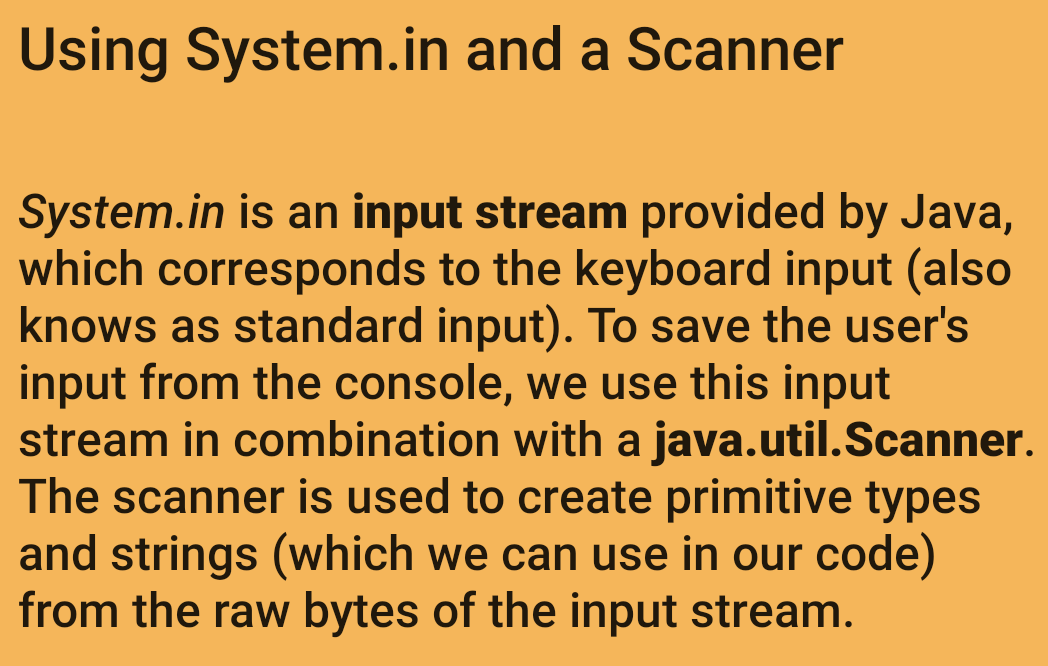
\includegraphics[width=5cm]{title_text_component}
		\caption{Részlet az \textit{input beolvasása} fejezetből (angol változat): címsor és szöveg.}
		\label{title_component_figure}
	\end{figure}
	
	Már ezzel a két komponenssel meg lehet jeleníteni a tananyag nagy részét, de azért hogy a fejezetek kevésbé legyenek monotonok, további komponenseket is implementáltam, melyek "megtörik" a szöveget. 
	
	\subsection{Bekeretezett szöveg}
	
	Ez a komponens lényegében egy szövegdoboz, ami eltérő háttérszínnel és saját címmel rendelkezik, ezáltal jobban felhívja a felhasználó figyelmét. Definiálása a $<boxed>$ taggel történik:
	
	\bigskip
	\begin{lstlisting}[language=XML]
	<boxed title="[Szövegdoboz címe]">
	<![CDATA[
	[Formázott szöveg]
	]]>
	</boxed>	
	\end{lstlisting}
	\bigskip
	
	Például a metódusok fejezetben ilyen szövegdobozba raktam a visszatérési érték nélküli metódusokkal kapcsolatos részt. Ezt lásd a \ref{boxed_component_figure} ábrán.
	
	\begin{figure}[h!]
		\centering
		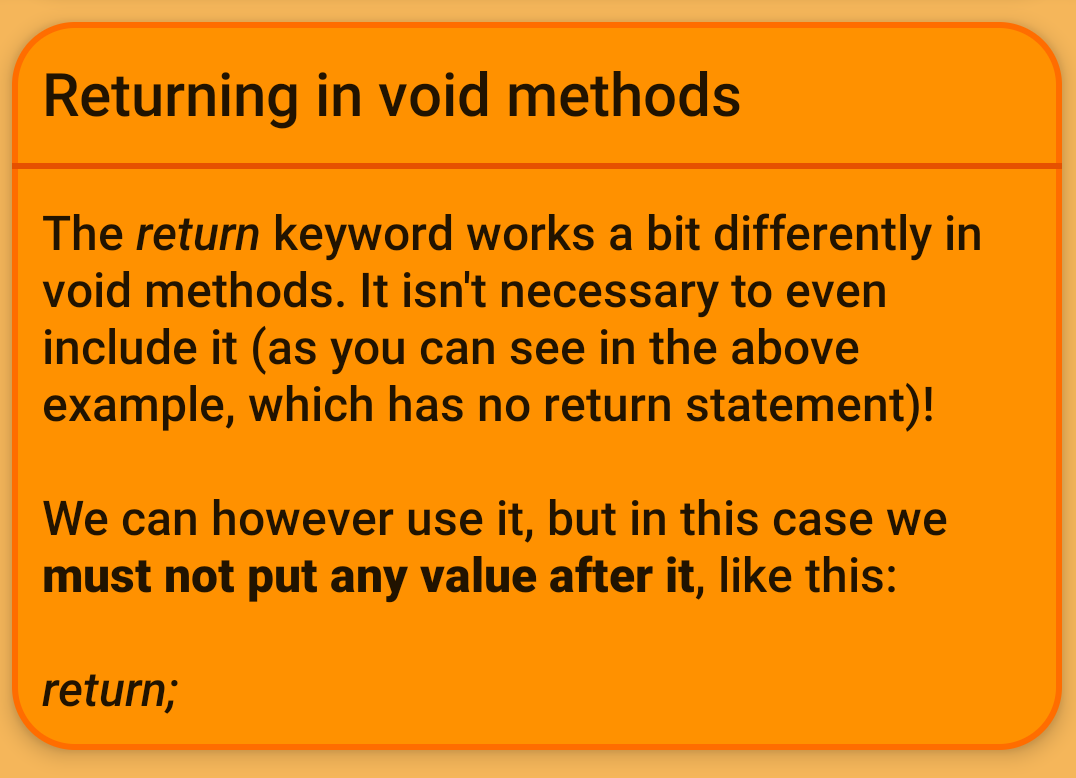
\includegraphics[width=5cm]{boxed_component}
		\caption{Részlet a \textit{Metódusok} fejezetből (angol változat): bekeretezett szöveg.}
		\label{boxed_component_figure}
	\end{figure}
	
	\subsection{Magas szintű tartalom}
	
	Ez a komponens hasonló a bekeretezett szöveghez, viszont speciálisan a nehezebb anyagrészek, kiegészítő információk megjelenítésére terveztem. Az $<advanced>$ taggel adható meg. Élénkpiros színnel fog megjelenni, és a felhasználó tudomására hozza, hogy az adott tartalom nehezebb, vagy csak egy későbbi kurzusban kerül részletes bemutatásra.
	
	\bigskip
	\begin{lstlisting}[language=XML]
	<advanced title="[Cím]">
	<![CDATA[
	[Formázott szöveg]
	]]>
	</advanced>	
	\end{lstlisting}
	\bigskip
	
	Ilyen jelzővel láttam el például a \textit{absztrakt osztályok és interfészek} fejezetben azt a rész, ahol a megemlítem, hogy milyen változásokon mentek keresztül az interfészek a \textit{Java 8} megjelenésével (\ref{advanced_component_figure}. ábra). Ez részletesebben egy későbbi kurzusban, a \textit{Java 8} nevűben van leírva.
	
	\begin{figure}[h!]
		\centering
		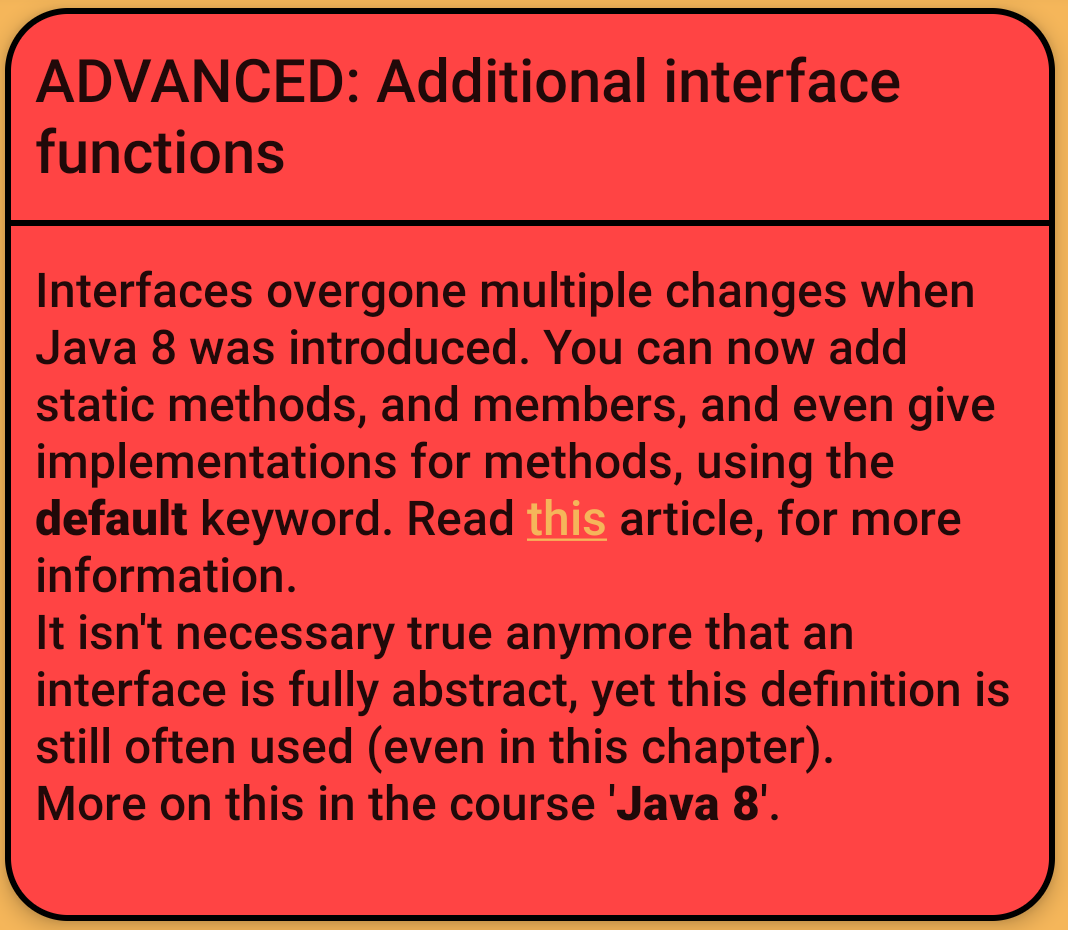
\includegraphics[width=5cm]{advanced_component}
		\caption{Részlet a \textit{Interfészek} fejezetből (angol változat): magas szintű tartalom.}
		\label{advanced_component_figure}
	\end{figure}
	
	Ebben a komponensben még egy link is található, ami a megfelelő oldalra viszi a felhasználót (a telefon alapértelmezett böngészőjében).
	
	\subsection{Képek}
	
	Lehetőség van képek beillesztésére a fejezetekbe és feladatokba, az $<image>$ tag segítségével. Egy attribútumban kell megadni, hogy melyik kép jelenjen meg. Arról, hogy hol tárolom a tananyagban felhasznált képeket részletesen a \ref{tananyag_tarolasa} részben írok. Az \xml struktúra a következőképpen néz ki:
	
	\bigskip
	\begin{lstlisting}[language=XML]
	<image name="[Kép neve]"/>
	\end{lstlisting}
	
	Például \textit{tömbök} fejezetben a több dimenziós tömbök megértését képpel segítettem elő, amint az a \ref{image_component_figure}. ábrán látható.
	
	\begin{figure}
		\centering
		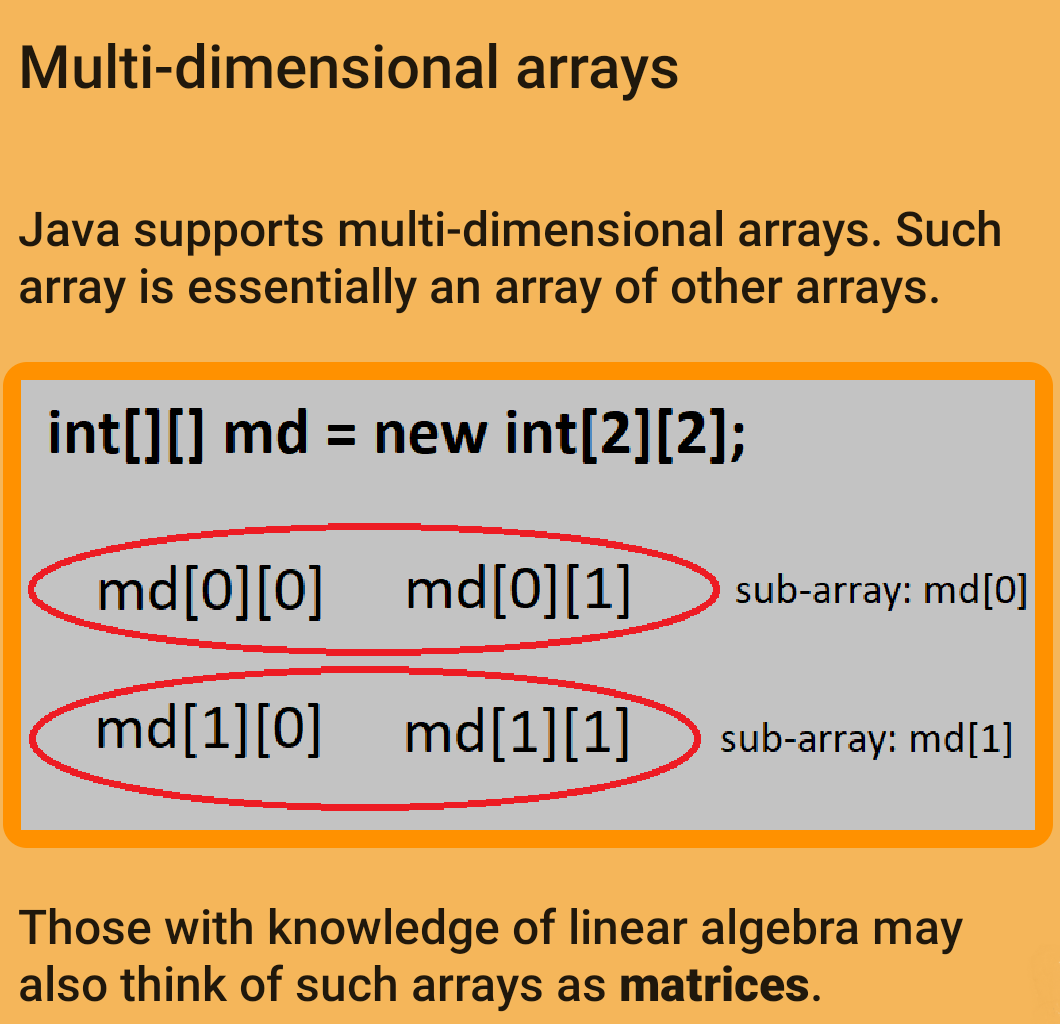
\includegraphics[width=5cm]{image_component}
		\caption{Részlet a \textit{Tömbök} fejezetből: grafikus tartalom.}
		\label{image_component_figure}
	\end{figure}
	
	\subsection{Kódminták} \label{kodmintak}
	
	A programozás oktatásánál elengedhetetlen, hogy kódrészletekkel segítsük a megértést. Az alkalmazásban lévő mintáknak egységes formázásúnak kell lenniük. Ezt úgy értem el, hogy előre definiáltam a színeket, amelyekkel a kód részeit kijelöltem. A következők kaptak saját kijelölőszínt:
	
	\begin{itemize}
		\item A \textit{Java} nyelv kulcsszavai.
		\item A \textit{Java} nyelv primitívei. Ide soroltam a \textit{void}-ot is, habár az valójában csak kulcsszó.
		\item Szöveg és karakter konstansok.
		\item Numerikus konstansok.
		\item Osztálynevek.
		\item Metódusok és adattagok nevei.
		\item Annotációk.
		\item Kommentek. 
	\end{itemize}
	
	A megjelenő kódmintáknak ugyanolyan sortörésekkel és tabulálással kell megjelenni az alkalmazásban, mint ahogy megírásra kerültek. Ezért a minták szövegébe a sorok végére $<br>$ sortörő taget kell elhelyezni, és a tabulálást pedig a $\&nbsp;$ szimbólummal kellet jelölni. A korábban bemutatott komponenseknél ez nem volt lényeges, ezeket az Android rendszer úgy tördelheti, ahogy a képernyő méretei megengedik, azonban a kódmintáknál fontos a helyes tördelés.
	
	További formázást igényelt, hogy a \textit{HTML} nyelv esetén a $<$ szimbólumot speciálisan kell jelölni, hogy az értelmező ne vegye egy új tag kezdetének. A megoldás az $\&lt$ karaktersorozattal történő helyettesítés. Ezért az olyan kódminták, melyek például összehasonlítást tartalmaznak mind külön formázást igényelnek.
	
	Látható, hogy rengeteg formázási szabályt vezettem be. Ha ehhez hozzávesszük a kódminták nagy számát, akkor látszik, hogy a manuális formázás nem célszerű. Ezért erre  célra egy külön formázó programot készítettem, ami egy megadott mappában lévő \textit{Java} kódot átalakít olyan \textit{HTML} kóddá, ami a fent említett összes szabálynak eleget tesz. Ez a program reguláris kifejezések alapján azonosítja a listában látható kifejezéseket és elhelyezi körülöttük a színezést és a tördelést biztosító tageket.  
	
	A fejezetekben és feladatokban kódmintát a $<code>$ tag segítségével definiálok. A tag belsejébe kell helyezni, azt a formázott kódot, amit az előző részben említett segédprogram ad eredményül.
	
	\bigskip
	\begin{lstlisting}[language=XML]
	<code>
	<![CDATA[
	[Formázott kód]
	]]>
	</code>	
	\end{lstlisting}
	\bigskip
	
	A megjelenítésnél nehézséget okoz, hogy a kódmintákban kosszú sorok lehetnek, amelyen nem minden eszköz képernyőjén férnek el egy sorban, viszont a mintákat a rendszer nem tördelheti szabadon. Ezért az alkalmazás kódmintái vízszintesen görgethetőek, ha vannak bennül olyan sorok, amelyek nem férnek el a képernyőn.
	
	\begin{figure}
		\centering
		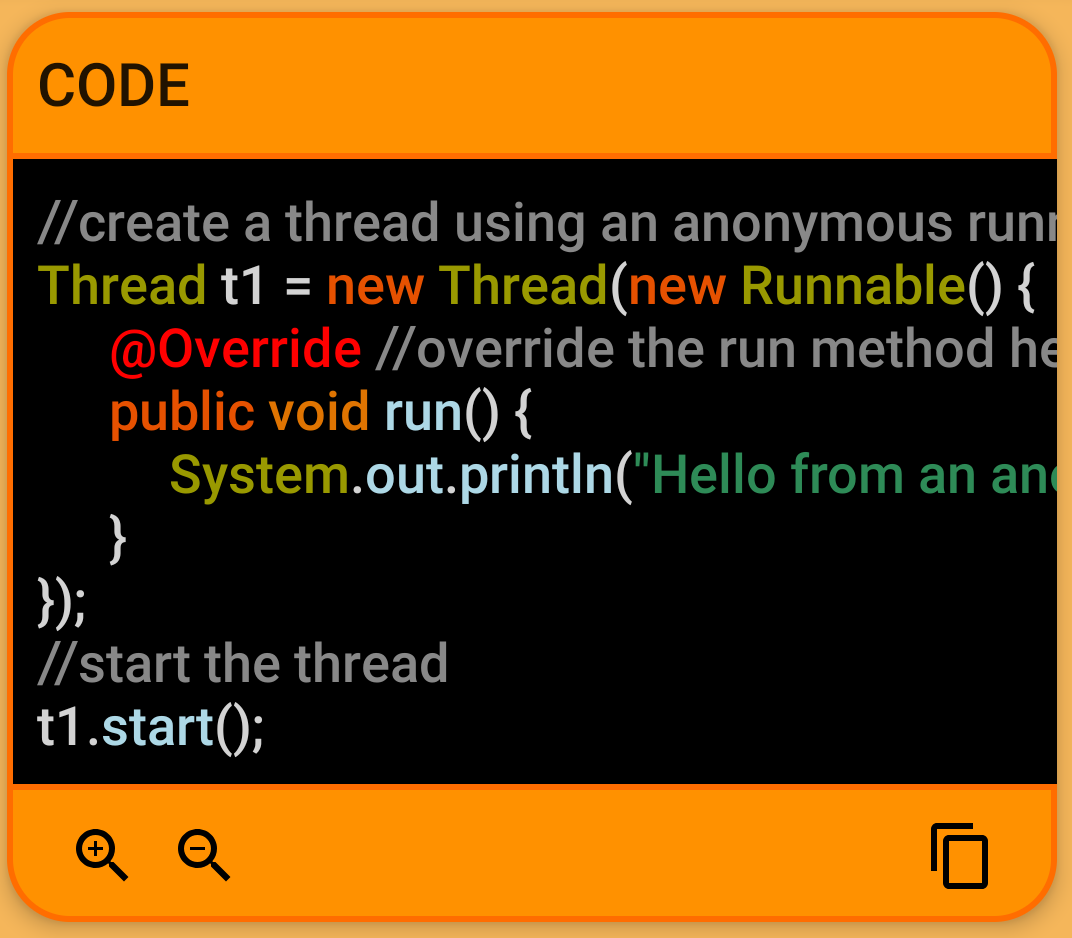
\includegraphics[width=5cm]{code_component_1}
		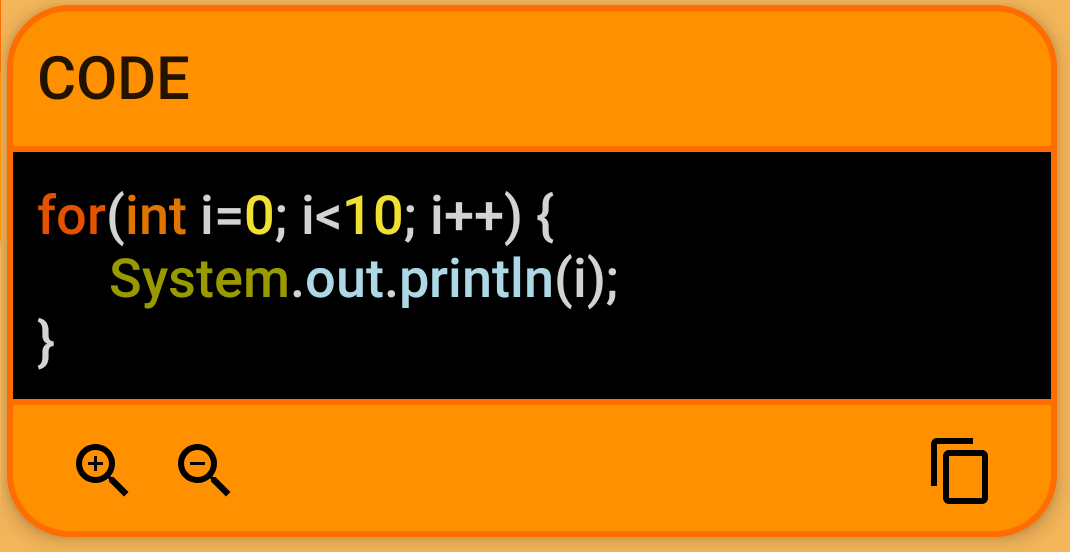
\includegraphics[width=5cm]{code_component_2}
		\caption{Kódminták az alkalmazásból (angol változat).}
		\label{code_component_figure}
	\end{figure}
	
	Megjelenített kódmintákért lásd a \ref{code_component_figure}. ábrát. A képek bal alsó sarkában lévő ikonokkal a kódminták betűmérete állítható. A jobb alsó sarokban lévő gomb aktiválja a \textit{ClipSync} funckiót, melyről részletesebben a \ref{clipsync} részben írok.
	
	\subsection{Interaktív kódminták}\label{interaktiv_kodmintak}
	
	Azért, hogy a tananyagot interaktívabbá tegyem, implementáltam a kódmintáknak olyan változatát is, ahol egyes szavak, vagy kifejezések hiányosak, kitöltésüket a felhasználó egy feladatkiírás alapján elvégezheti. Ez a komponens is \xml-ben van definiálva, és formázott kódot vár. A formázás folyamatáról a \ref{kodmintak_formazas}. részben írtam.
	
	Az interaktív kódmintának meg kell adni, hogy hol legyenek benne módosítható részek, mezők, melyek tartalmát a felhasználó átírhatja. Ezek megadásához a formázott kódba három alulvonás jelet kell beszúrni. Ahol a beolvasás során ezt a karaktersorozatot találja az alkalmazás, oda egy módosítható rész fog kerülni. Például így lehet megjeleníteni egy változódeklarálást, ahol a változó értéke módosítható lesz:
	
	\bigskip
	\begin{lstlisting}[language=Java]
	int x = ___ ;
	\end{lstlisting}  
	\bigskip
	
	Az olvashatóság miatt itt nem tüntettem fel a formázást, egy valódi minta esetén \textit{HTML} tagek is szerepelnek a formázott kódban.
	
	A mezők azonosítása indexelés alapján történik. Mindegyik mezőhöz meg kell adni, hogy oda milyen megoldásokat vár az alkalmazás. Szintén megadható alapértelmezett tartalom, ilyenkor az adott mező nem üresen, hanem a megadott tartalommal jelenik meg. Ez felhasználható például olyan interaktív minta megadására, ahol a felhasználó dolga a kódrészlet kijavítása, nem pedig egyszerűen a kitöltése.
	
	Az interaktív kódmintákat a következő \xml struktúrával lehet megadni:
	
	\bigskip
	\begin{lstlisting}[language=XML]
	<interactive instruction=[Kitöltési instrukció]>
	<data>
	[Formázott kód, mezőket jelölő karakterekkel]
	</data>
	<answer place=[Index]>[Válasz]</answer>
	...
	<answer place=[Index]>[Válasz]</answer>
	</interactive>
	\end{lstlisting}
	\bigskip
	
	Egy indexhez több $<answer>$ tag is tartozhat, ilyenkor az adott mezőnek több megoldása is van. Az opcionális alapértelmezett tartalmakat $<default>$ tagek közt kell megadni:
	
	\bigskip % Ide nem írok language jelölőt, mert valamiért kijelöli a default szót
	\begin{lstlisting}
	<default place=[Index]>[Alapértelmezett érték]</default>
	\end{lstlisting}
	\bigskip
	
	Amikor a fent megadott módon elkezdtem az interaktív minták megírását, hamar rájöttem, hogy ez az eszköztár sokszor még a legegyszerűbb feladatok megadásához is kevés. Vegyük a következő példát:
	
	Az utasítás az, hogy egészítsük ki a kapott kódmintát, méghozzá úgy, hogy a változó végső értéke legyen 8!
	
	\bigskip
	\begin{lstlisting}[language=Java]
	int num = ___ ;
	num = num ___ 5 ;
	\end{lstlisting}  
	\bigskip
	
	Látható, hogy több megoldás is van:
	
	\begin{itemize}
		\item Az első mezőbe 3, a másodikba \textit{+} beírásával az eredmény 8 lesz.
		\item A 13 és a \textit{-} jel kombinációja is helyes.
		\item Nyolcat kapunk továbbá a 40 és a \textit{/} megadásával is.
	\end{itemize}
	
	A probléma azonban nem oldható meg annyival, hogy lehetséges megoldásként az első mezőhöz felvesszük a 3, 13 és 40 értékeket, a másodikhoz pedig a \textit{+}, \textit{-} és \textit{\%} szimbólumokat. Ebben az esetben ugyanis ezek helytelen kombinációját is elfogadná az alkalmazás, pedig csak a listában megadott kombinációk helyesek.
	
	Ezt a nehézséget úgy hidaltam át, hogy csoportosíthatóvá tettem a válaszokat. Egy csoportba tartozó válaszok csak együtt lesznek elfogadva. Az előző példa válaszait így a következőképpen lehet elkódolni:
	
	\bigskip
	\begin{lstlisting}
	<answer place="0" group="add">3</answer>
	<answer place="1" group="add">+</answer>
	<answer place="0" group="subtract">13</answer>
	<answer place="1" group="subtract">-</answer>
	<answer place="0" group="div">40</answer>
	<answer place="1" group="div">/</answer>
	\end{lstlisting}
	\bigskip
	
	Példák alap és javított állapotban lévő kódmintákról a \ref{interactive_component_figure}. és a \ref{interactive_component_completed_figure}. ábrákon láthatóak. 
	
	\begin{figure}
		\centering
		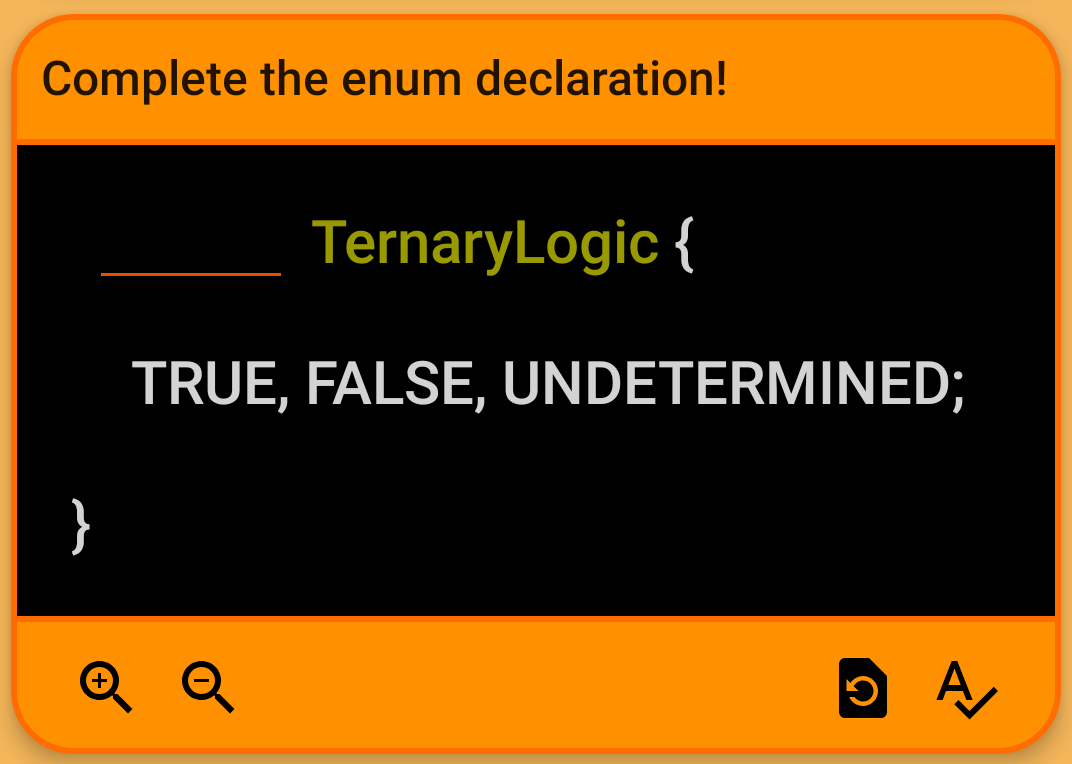
\includegraphics[width=5cm]{interactive_not_completed}
		\caption{Interaktív kódminta az alkalmazásból (angol változat).}
		\label{interactive_component_figure}
	\end{figure}
	
	\begin{figure}
		\centering
		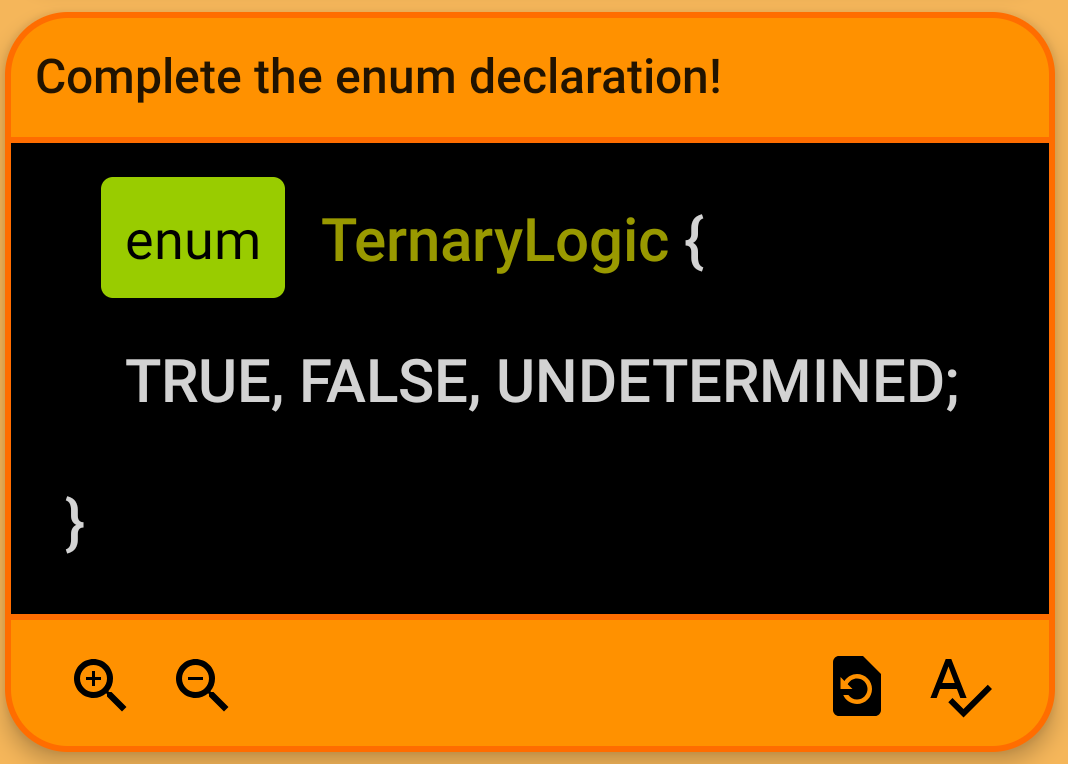
\includegraphics[width=5cm]{interactive_correct}
		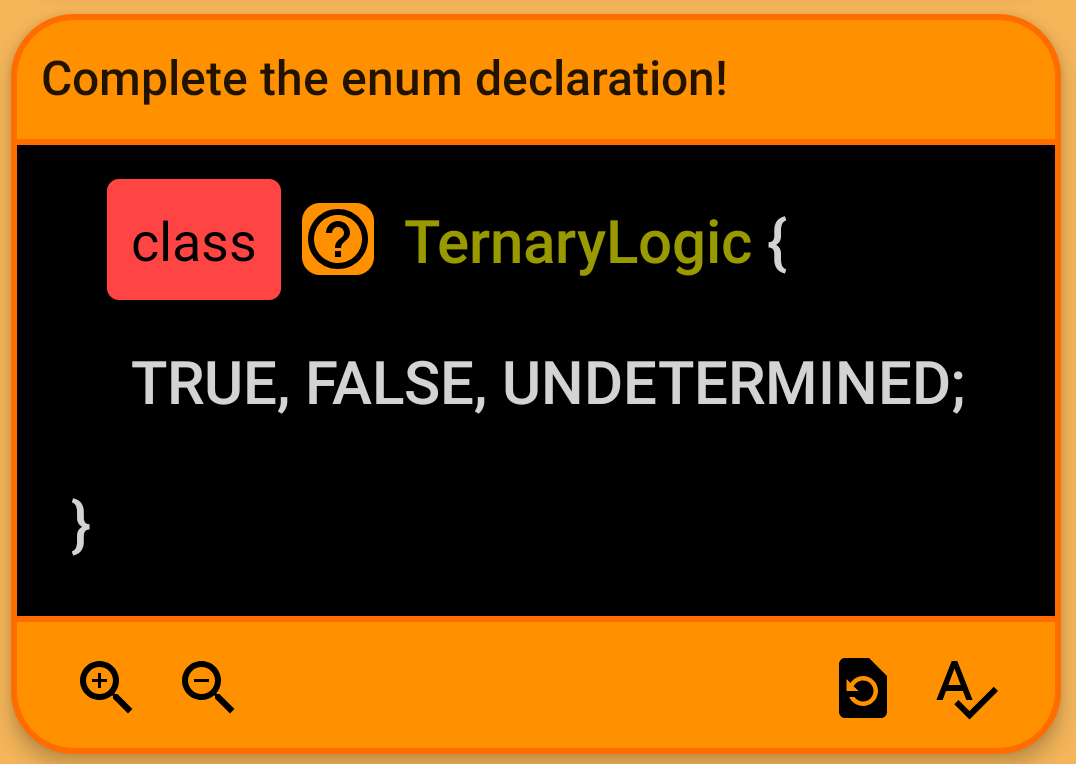
\includegraphics[width=5cm]{interactive_incorrect}
		\caption{A \ref{interactive_component_figure}. ábrán látható interaktív kódminta, javítva (angol változat).}
		\label{interactive_component_completed_figure}
	\end{figure}
	
	A bal alsó sarokban lévő ikonok a \ref{kodmintak} fejezetből már ismert betűméret állítók, a jobb alsó sarokban lévő gombokkal pedig a felhasználó elkérheti a megoldást, vagy alaphelyzete állíthatja a komponenst. A helyes és helytelen megoldások kijelölésre kerülnek. A helytelen megoldásnál megfigyelhető kérdőjel ikon segítségével el lehet kérni az adott mező helyes megoldását, arra az esetre, ha a felhasználó elakadna.
	
	\subsection{Kérdések}\label{kerdesek}
	
	A kérdések hasonló elven működnek, mint a fejezeteben megjelenő komponensek, a kérdések azonban csak a vizsgákban fordulnak elő. Szintén \xml-ben vannak definiálva.
	
	Míg a fejezeteket és feladatokat megadó \xml fájlokban minden komponens felhasználásra kerül, méghozzá a megadott sorrendben, addig a vizsgákat definiáló fájlokban a kérdések sorrendje nem számít, és az sem biztos, hogy mind meg is fog jelenni. Ennek oka a változatosság. Ha egy vizsga megnyitásakor mindig ugyanazok a kérdések, ugyanabban a sorrendben jelennének meg, az kiszámítható lenne.
	
	Ennek elkerülésére az alkalmazás a vizsga megnyitásakor az \xml értelmezése után egy véletlenszerű, előre megadott méretű listát állít össze a kérdésekből. Az egy vizsgához tartozó kérdés mennyiség szintén a vizsgát leíró \xml-ben van megadva, ez jellemzően 20-25 kérdés.
	
	Ahogy a fejezetekben megjelenő komponenseknek, úgy a kérdéseknek is több típusa van. Ennek oka egyrészt a monotonitás megtörése, másrészt a különböző kérdéstípusok lehetőséget adnak a vizsga készítőjének, hogy sokféle kérdést fel tudjon tenni. Például, ha csak feleletválasztós kérdés lenne, akkor nem lehetne olyan kérdést feltenni, amiben írásos választ várunk.
	
	Minden kérdéstípusnak automatikusan javíthatónak kell lennie, hogy az alkalmazás ki tudja értékelni az elkészült vizsgát. Ez kizárja az olyan kérdéseket, amik hosszú szöveges választ várnak (esszé).
	
	Minden kérdéstípusban közös, hogy tartalmazza a kérdés szövegét, a lehetséges és a helyes megoldásokat. Az azonban, hogy ezek minként vannak elkódolva, már az egyes fajtáktól függ. Most bemutatom a támogatott kérdéstípusokat.
	
	\subsubsection{Feleletválasztós kérdés egy válaszlehetőséggel}
	
	Ez a kérdéstípus tetszőleges számú lehetséges választ tud megjeleníteni, amelyek közül a felhasználó egyet jelölhet meg helyesként. Alap állapotában egyik válasz sincs megjelölve. A következőképpen van \xml-ben definiálva:
	
	\bigskip
	\begin{lstlisting}[language=XML]
	<question type="single_choice">
	<text>[A kérdés szövege]</text>
	<answer>[Lehetséges válasz]</answer>
	...
	<answer>[Lehetséges válasz]</answer>
	<correct>[Helyes válasz száma]</correct>
	</question>
	\end{lstlisting}
	\bigskip
	
	Minden $<answer>$ tag elkódol egy lehetséges megoldást, a $<correct>$ tag pedig ezek közül a helyes válasz (0-tól számolt) indexe. Én jellemzően olyan kérdéseket írtam, ahol 3-4 válaszlehetőség van. 
	
	Az, hogy miként jelennek meg az alkalmazásban ezek a kérdések, a \ref{question_single_choice_figure} ábrán látható.
	
	\begin{figure}[h!]
		\centering
		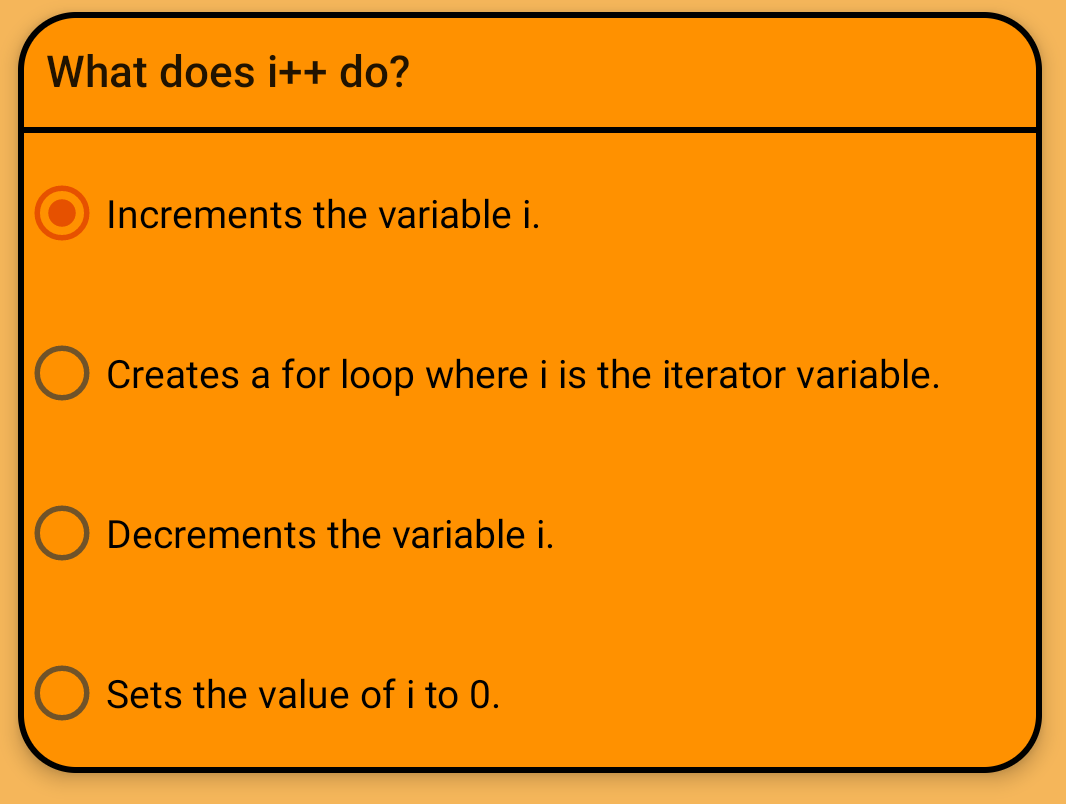
\includegraphics[width=5cm]{question_single_choice}
		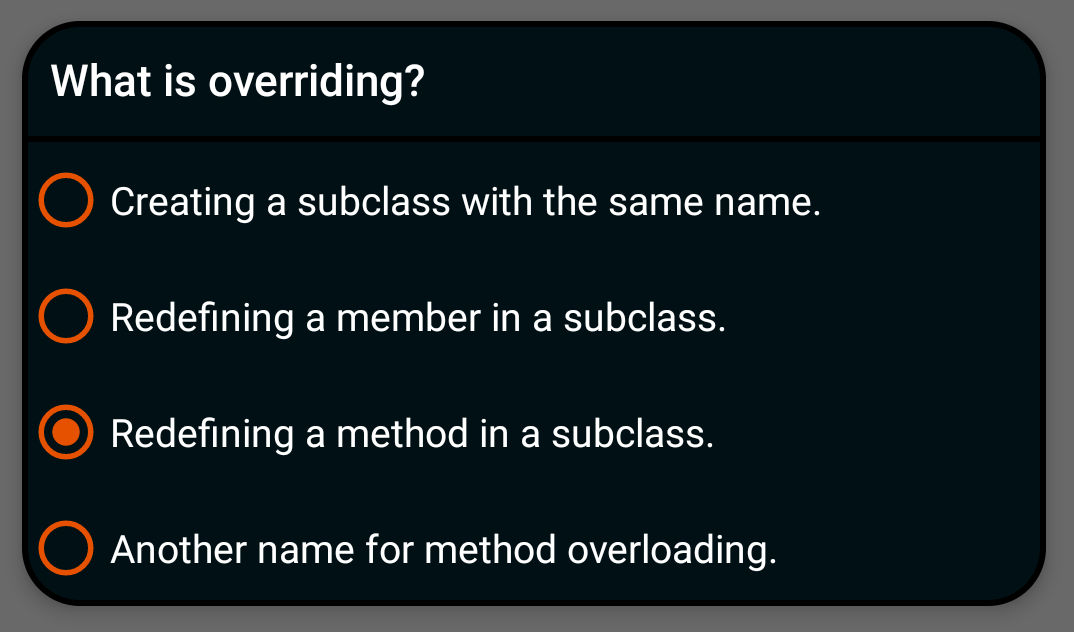
\includegraphics[width=5cm]{question_single_choice_dark}
		\caption{Feleletválasztós kérdések az alkalmazás angol változatából, normál és sötét témában.}
		\label{question_single_choice_figure}
	\end{figure}
	
	\subsubsection{Feleletválasztós kérdés több válaszlehetőséggel}
	
	Egy újabb feleletválasztós típus, éppen ezért sokban hasonlít a fent ismertettet egy választási lehetőséggel rendelkező kérdésre. A különbség, hogy ebben az esetben a felhasználó a megjelenített lehetséges válaszok közül bármyennyit megjelölhet helyesként.
	
	Az elkódolás ennek megfelelően változik. Több $<correct>$ tag is megjelenhet, de egyébként pontosan ugyan olyan, mint az egy választási lehetőséggel rendelkező kérdések esetén. Megjelenített kédések több válaszlehetőséggel a \ref{question_multi_choice_figure}. ábrán láthatóak.
	
	\begin{figure}[h!]
		\centering
		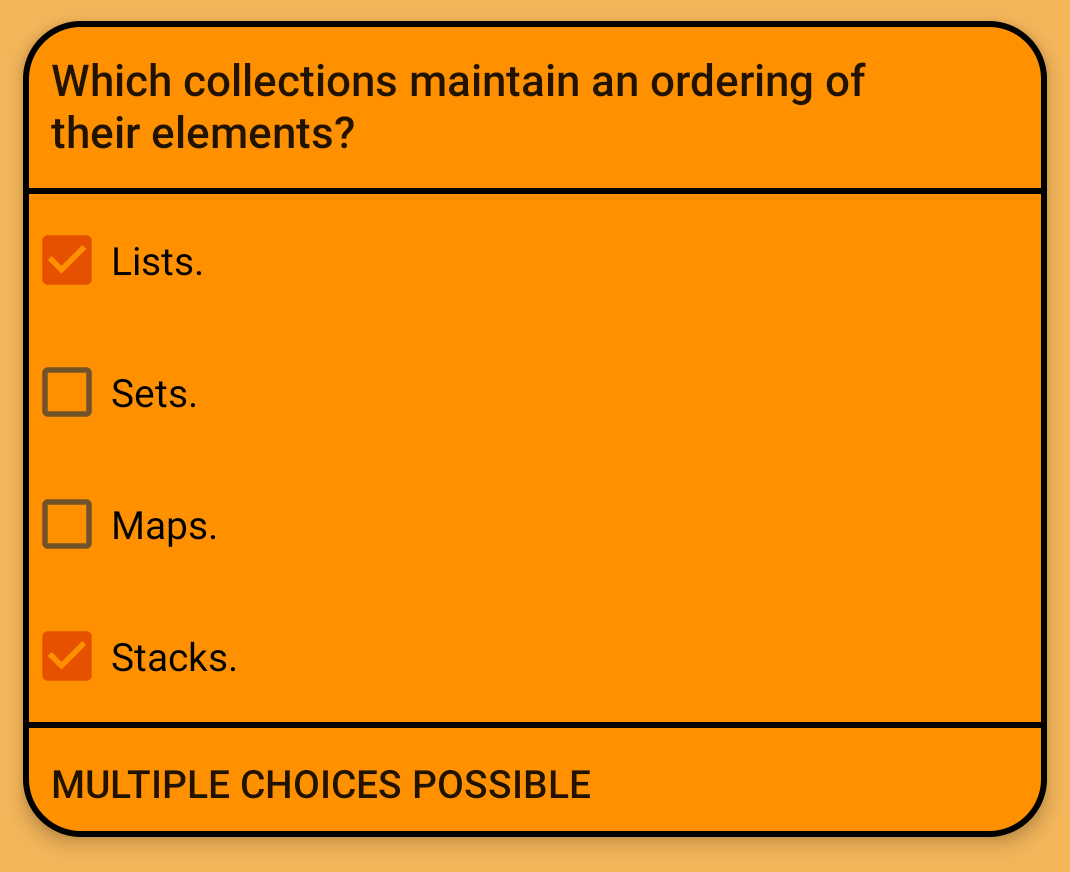
\includegraphics[width=5cm]{question_multi_choice}
		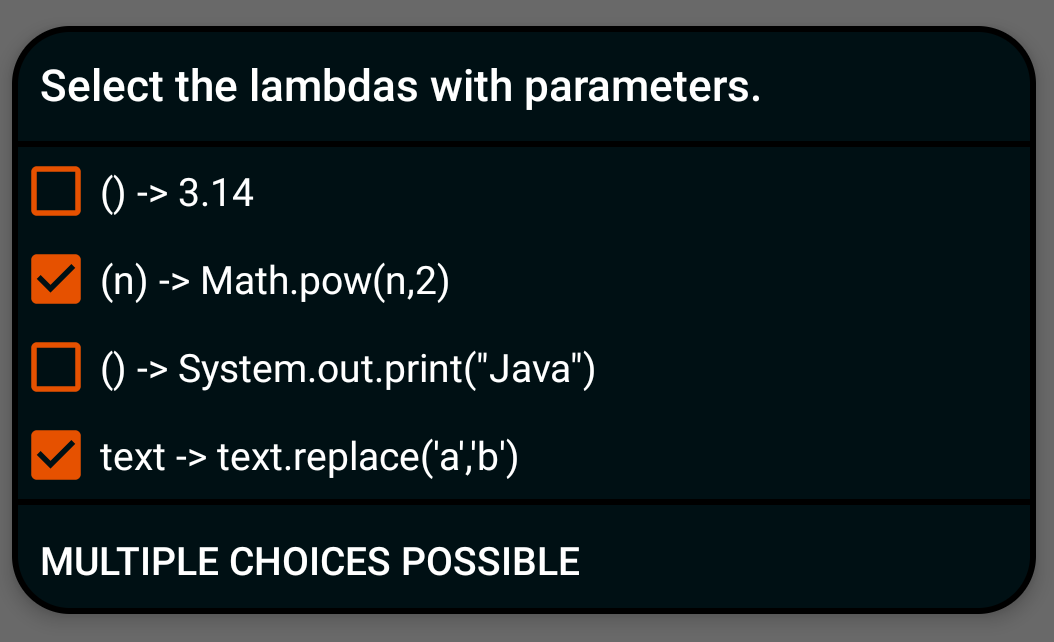
\includegraphics[width=5cm]{question_multi_choice_dark}
		\caption{Több válaszlehetőséges kérdések az alkalmazás angol változatából, normál és sötét témában.}
		\label{question_multi_choice_figure}
	\end{figure}
	
	\subsubsection{Szöveges kérdés}\label{question_text}
	
	A legösszetettebb kérdéstípus, ami szöveges választ vár a felhasználótól. \xml elkódolása (egyszerű esetben) a következő:
	
	\bigskip
	\begin{lstlisting}[language=XML]
	<question type="text">
	<text>[A kérdés szövege]</text>
	<correct>[Elfogadott szöveges válasz]</correct>
	...
	<correct>[Elfogadott szöveges válasz]</correct>
	</question>
	\end{lstlisting}
	\bigskip
	
	\noindent
	Megfigyelhető, hogy itt nincsen $<answer>$ tag, mivel ez a kérdéstípus nem mutat lehetséges válaszokat a felhasználónak. $<correct>$ tagből több is támogatott, mindegyik esetén pontos egyezés lesz szükséges a felhasználó válaszával, hogy az el legyen fogadva.
	
	Amikor elkezdtem ténylegesen kérdéseket írni, rájöttem, hogy ez a fajta validáció rugalmatlan, és nagyon hosszú kérdés definíciókat eredményez. Például szeretném megkérdezni a felhasználótól, hogy \textit{minek a rövidítése a JDK}. A válasz persze \textit{Java Development Kit}, de mi történjem, ha a vizsgázó ezt kis betűkkel írja le, vagy esetleg csak az első szó lesz nagybetűs. Szerettem volna ezeket mind elfogadni, mivel teljesen helyes válaszok, ehhez azonban nagyon sokféle helyes választ kellett definiálnom, és még így is előfordulhat, hogy a felhasználó által beírt válasz helyes, de éppen nem lesz köztük.
	
	A probléma megoldására hoztam létre a nagybetűt figyelmen kívül hagyó kérdést, amit az $<ignoreCase>$ tag elhelyezésével lehet megadni:
	
	\begin{lstlisting}[language=XML]	
	<question type="text">
	<text>Minek a rövidítése a JDK?</text>
	<correct>Java Development Kit</correct>
	<ignoreCase/>
	</question>
	\end{lstlisting}
	
	\noindent
	Egy sokkal nehezebb problémával szembesültem, amikor olyan kérdéseket kezdtem írni, amelyek valamilyen kódrészlet megadását kérik. Vegyük azt a példát, ahol adott egy $i$ nevű változó, és azt kérjük a felhasználótól, hogy írjon utasítást, ami ennek a változónak a $4$ értéket adja. A helyes válasz persze $i = 4;$, de a szóközök gondot jelenthetnek. Korrekt megoldás az is, ha egyáltalán nem írunk szóközt az egyenlőség jel elé, vagy után, de a Java fordító azt is elfogadja, ha 20 szóközt írunk elé, vagy mögé.
	
	Logikusnak tűnik egy $<ignoreSpace>$ tag bevezetése, ami majd minden szóközt töröl a felhasználó válaszából, és csak utána veti össze a helyes megoldással. A fenti példát megoldaná, viszont könnyen találhatunk olyat, ahol ez nem kivitelezhető. Tegyük fel, hogy egy olyan utasításra akarunk rákérdezni, ami deklarál egy $int$ típusú $i$ változót, és az értékét $0$-ra állítja. Ez nyilván $int \ i = 0;$ lesz. Ha azonban erre alkalmaznánk a szóközöket kidobó ellenőrzést, akkor az elfogadná a $inti=0;$ választ is, ami pedig érvénytelen.
	
	Ezt a nehézséget úgy oldottam meg, hogy a megoldásba elhelyezhetőek "fontos" szóközök, amiket az $<ignoreSpace>$ tag nem fog figyelmen kívül hagyni. Ha egy fontos szóköz hiányzik akkor a válasz nem lesz elfogadva. Itt látható a példa, ahol a fontos szóközöket jelölő $[s]$ karaktersorozatot illesztettem az $int$ és az $i$ közé:
	
	\begin{lstlisting}[language=XML]	
	<question type="text">
	<text>...</text>
	<correct>int[s]i = 0;</correct>
	<ignoreSpace/>
	</question>
	\end{lstlisting}
	
	\noindent
	Megjegyzem, hogy a két módosító tag együtt is használható, de ez jellemzően nem szükséges, mert ha kódrészletre kérdezünk, akkor az abban lévő kulcsszavak esetén csak a kisbetűs írásmód helyes. Megjelenített szöveges kérdések a \ref{question_text_figure}. ábrán láthatóak.
	
	\begin{figure}[h!]
		\centering
		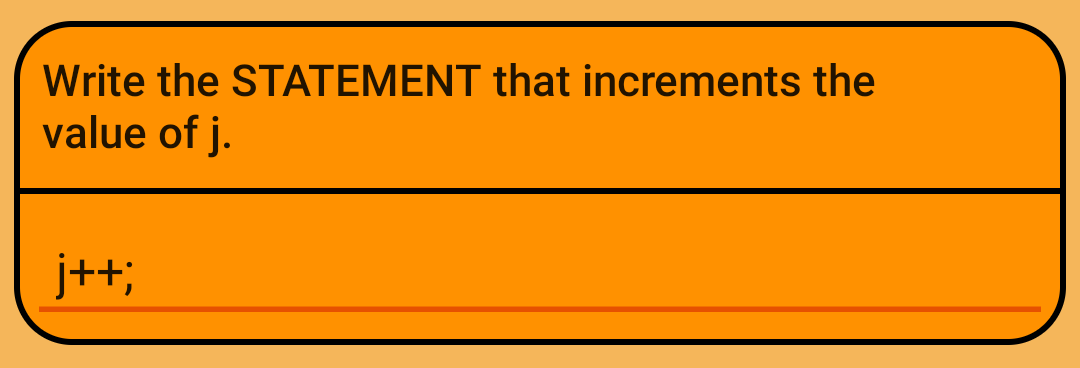
\includegraphics[width=5cm]{question_text}
		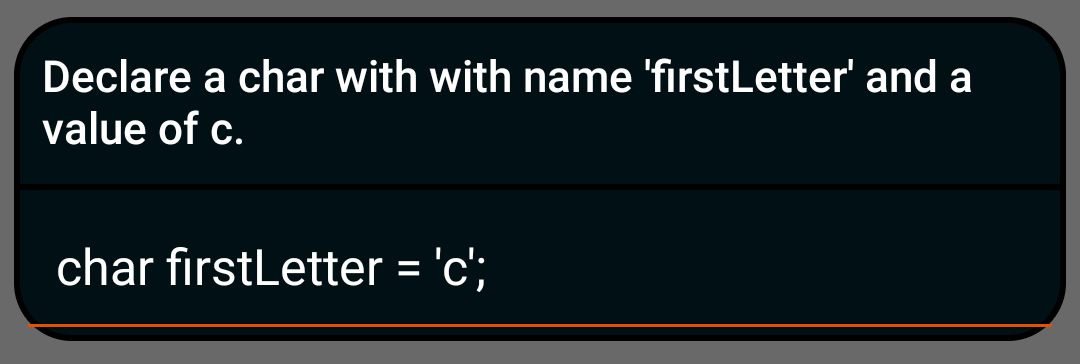
\includegraphics[width=5cm]{question_text_dark}
		\caption{Szöveges kérdések az alkalmazás angol változatából, normál és sötét témában.}
		\label{question_text_figure}
	\end{figure}
	
	\subsubsection{Igaz-hamis kérdés}
	
	A kérdések írása során rengetegszer előjött az olyan feleletválasztós kérdés, ahol a két lehetséges válasz mindössze az $igaz$ és a $hamis$ volt. Erre az esetre külön típust készítettem, egyrészt azért, hogy a kérdés definíciója egyszerűsödjön, másrészt pedig, hogy a felhasználó számára is világosan látszódjon, hogy itt igaz-hamis kérdésről van szó. \xml elkódolása így néz ki:
	
	\begin{lstlisting}[language=XML]	
	<question type="true_false">
	<text>[A kérdés szövege]</text>
	<correct>[Itt 'true' vagy 'false' állhat]</correct>
	</question>
	\end{lstlisting}
	
	Ez a kérdéstípus a feleletválasztós helyett két gombot jelenít meg, ahogy az a \ref{question_true_false_figure}. ábrán látható.
	
	\begin{figure}[h!]
		\centering
		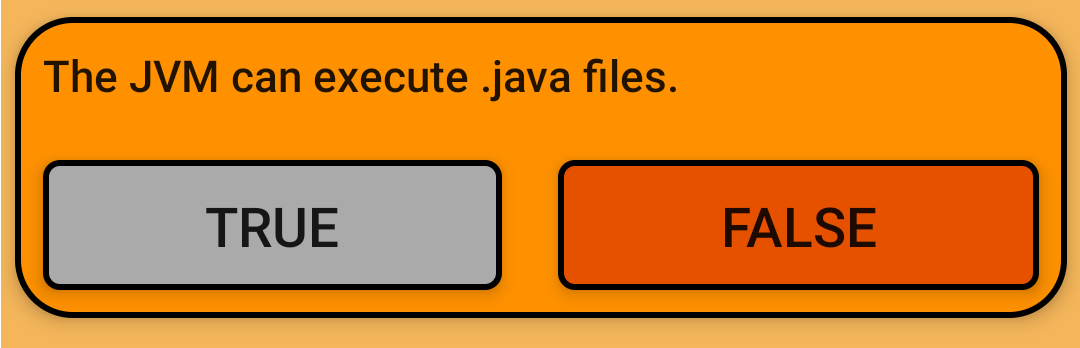
\includegraphics[width=5cm]{question_true_false}
		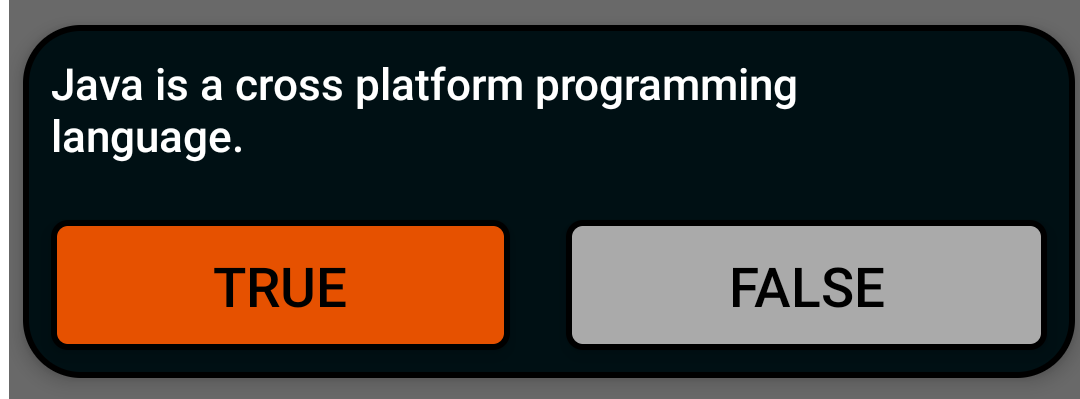
\includegraphics[width=5cm]{question_true_false_dark}
		\caption{Igaz-hamis kérdések az alkalmazás angol változatából, normál és sötét témában.}
		\label{question_true_false_figure}
	\end{figure}
	
	\subsubsection{A kérdések kiértékelése}
	
	Az alkalmazás kiértékeli a felhasználó által megadott válaszokat, ami alapján pontszámot rendel a vizsgához. A vizsga kiértékelését több minden is okozhatja: a felhasználó megnyomja a befejezés gombot, lejár az idő, megszakad a vizsga.
	
	A pontozásnál nagyon egyszerű szabályt követtem: minden helyes kérdés egy pontot ér, a helytelen nullát, nincsenek részpontok. Az, hogy mi számít helyesnek, a kérdés típusától függ. Egy választási lehetőséges illetve igaz-hamis kérdések esetén ez triviális. Több válaszlehetőséges kérdésnél akkor lesz helyes a válasz, ha a felhasználó megjelölt minden jó választ, és nem jelölt meg egy rosszat sem. Szöveges válasz esetén alapból pontos egyezésre van szükség, de azok a kérdések, melyek $<ignoreCase>$ vagy $<ignoreSpace>$ tagekkel vannak jelölve speciális módon értékelődnek ki, ahogy arról a szöveges kérdés fejezetben (\ref{question_text}) írtam.
	
	Minden egyes kérdés megjeleníti a javítás eredményét. A jó válaszokat zöld színnel, a hibásakat pirossal emeltem ki. Azoknál a kérdés típusoknál, ahol látszódnak a lehetséges válaszok, ott ez a javítás egyértelművé teszi a felhasználó számára, hogy hol hibázott, és mi lett volna a helyes megoldás. A szöveges kérdésnél azonban nincsenek megjelenítve lehetséges válaszok, így ha ezt a vizsgázó elrontotta, akkor mutatok egy helyes választ is.
	
	Azt bemutatni, hogy miként néz ki minden kérdéstípus javítás után, helyes és helytelen megoldással túl sok képet eredményezne, de a \ref{corrected_questions}. ábrán látható néhány javított kérdés.
	
	\begin{figure}[h!]
		\centering
		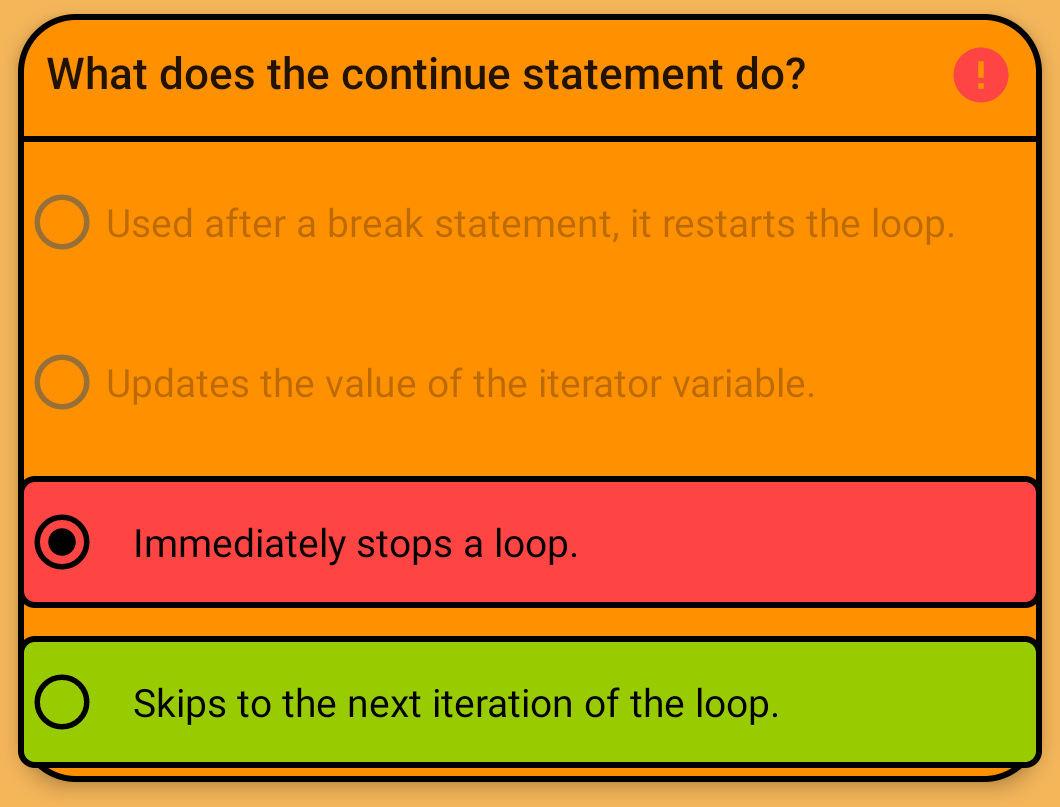
\includegraphics[width=5cm]{corrected_question_1}
		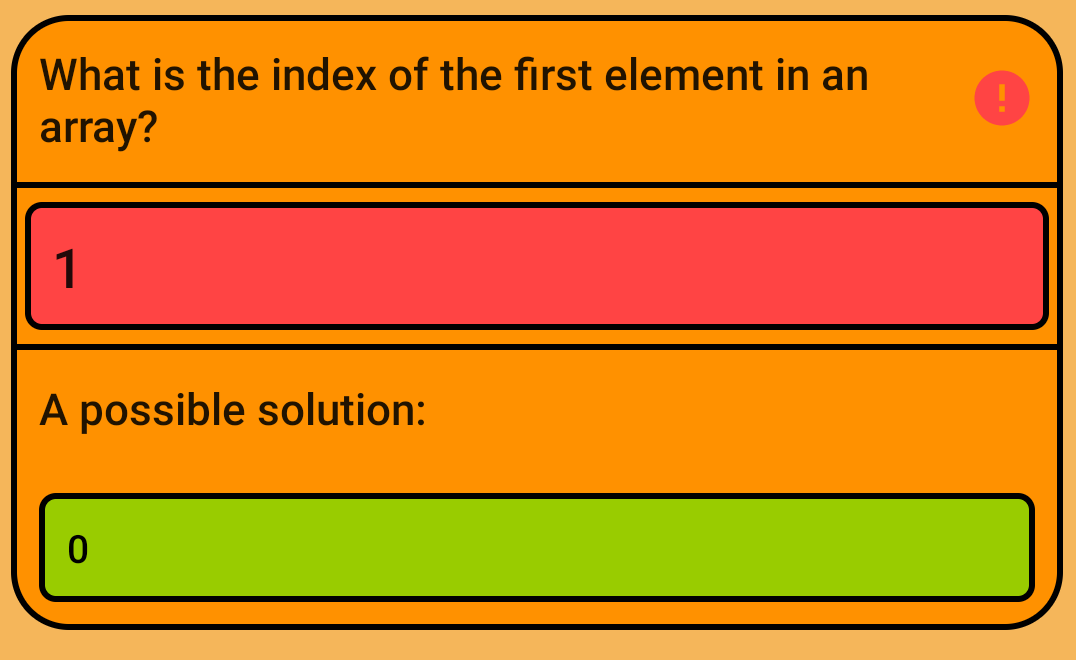
\includegraphics[width=5cm]{corrected_question_2}
		\caption{Javított kérdések, ahol a felhasználó hibás választ adott meg.}
		\label{corrected_questions}
	\end{figure}
	
	A vizsga befejeződésekor a kérdések egyéni javítása mellett megjelenik az összpontszám is, ami alapján az alkalmazás eldönti, hogy a vizsga sikeres volt-e, vagy sem. A beállításoknál lehetőség van az vizsgák nehézségének megadására, az itt megadott nehézség dönti el, hogy hány százalék elérésére van szükség a sikeres vizsgához.
	
	\section{Az Android alkalmazás felépítése}\label{android_alk_felepites}
	
	%\subsection{Beolvasási folyamat} --> kell-e ez?
	
	\subsection{A tananyag tárolása}\label{tananyag_tarolasa}
	
	A tananyagot a forráskódtól el kell különíteni, viszont futásidőben elérhetőnek kell lennie, hogy a felhasználó kéréseit ki lehessen szolgálni. Fontos az egységes elkódolás. Például minden kurzust leíró erőforrásfájlnak azonos felépítésűnek kell lennie: meg kell mondaniuk mely fejezetek, feladatok és vizsga tartozik hozzájuk.
	
	Az \textit{Android} alapelve, hogy az erőforrásfájlok legyenek elkülönítve a kódtól, és erre több eszközt is kínál. Az első a \textit{Resource System} (erőforrás rendszer). Ebben olyan erőforrásfájlok tárolhatóak, melyekre a legtöbb alkalmazásnak szüksége van:
	
	\begin{itemize}
		\item Grafikus elemek (\textit{drawable}): lehetnek ikonok, képek, hátterek, stb.
		\item Szövegek (\textit{string}): a felhasználói felületen megjelenő feliratok.
		\item Elrendezések (\textit{layout}): a felhasználói felület elrendezését tárolják.
		\item Még sok további előre definiált kategória: stílusok, színek, stb.
	\end{itemize} 

	Az erőforrás rendszer nem a legmegfelelőbb mód a tananyag tárolására, mivel az egyetlen gyakori, előre definiált kategóriába sem esik. Ennek ellenére az első verziókban az erőforrás rendszert használtam, mivel egyszerűen nem tudtam arról, hogy van jobb alternatíva.
	
	Biztosított továbbá az \textit{Asset System} (eszköz rendszer), mely annyiban tér el az előbb bemutatott erőforrás rendszertől, hogy itt nincsenek kategóriák, be tud fogadni bármilyen erőforrásfájlt, amelyre egy alkalmazásnak szüksége lehet. Ez tehát alkalmasabb módszer a tananyag tárolására, mint az erőforrás rendszer, és át is tértem ennek a használatára.
	
	Egy további érdekes lehetőség a tananyag tárolására egy szerver alkalmazás használata. A \textit{backend} biztosíthatna egy \textit{REST API}-t, amellyel az alkalmazás le tudná kérni a tananyag tartalmát. Ennek a módszernek az előnye, hogy így az alkalmazásból nem nyerhetőek ki a tananyagot alkotó \xml fájlok, mivel azok a szerveren vannak. Továbbá az alkalmazás mérete is csökkenne. Hátrány, hogy az alkalmazás alapvető használata internettől függővé válna, anélkül még egy fejezetet sem lehetne betölteni. 
	
	Valós lehetőségként ez a tárolási forma egyáltalán nem merült fel, mivel a tervezés során nem gondolkodtam szerver alkalmazásban.
	
	\subsection{Adatbázis}
	
	Az alkalmazásnak képesnek kell lennie eltárolnia felhasználó előrehaladását a tananyagban. A következő adatokat kell elmenteni:
	
	\begin{itemize}
		\item Teljesített vizsgák: Ez az információ a legfontosabb, mivel meghatározza, hogy melyik kurzusok elérhetőek.
		\item Elolvasott fejezetek: Mivel egy kurzus vizsgája csak akkor nyílik meg, ha a felhasználó minden fejezetet elolvas az adott kurzusból.
		\item Teljesített feladat: A feladatok teljesítése opcionális, de az alkalmazás ezt is eltárolja.
	\end{itemize}
	
	A \ref{tananyag_tarolasa} fejezetben említett \textit{Resource System} és \textit{Asset System} futásidőben csakis fájl olvasást tesznek lehetővé, írást nem. Ezért egy relációs adatbázist használok. \textit{NoSQL} adatbázis is lehetne, arról hogy miért a választott módszer mellett döntöttem, a \ref{sqlite_roon} fejezetben írok.
	
	Az előrehaladást a programban és az adatbázisban is egységesen jelölöm. Erre egy saját \textit{Java} annotációt használok:
	
	\begin{lstlisting}[language=Java]
@IntDef
public @interface Status {

	int LOCKED = 0;
		
	int UNLOCKED = 1;
		
	int COMPLETED = 2;
}
	\end{lstlisting}
	
	Az \textit{@IntDef} annotáció listázza, hogy mik lehetnek a lehetséges értékei egy olyan változónak, melyek \textit{@Status} annotációval látunk el. Ez fordítási időben ellenőrzésre kerül. Például ha a felhasználó először teljesít egy vizsgát, akkor annak státusza \textit{UNLOCKED}-ról \textit{COMPLETED}-re for változni az adatbázisban.
	 
	\subsubsection{Struktúra}\label{adatbazis_struktura}
	 
	Az adatbázis szerkezete egyszerű. A tananyag négy egységéhez (kurzus, fejezete, feladat, vizsga) rendel egy-egy táblát, és ezen táblák rekordjai tárolják az előrehaladást. Így néz ki az egyed-kapcsolat diagram:
	
	\begin{center}
		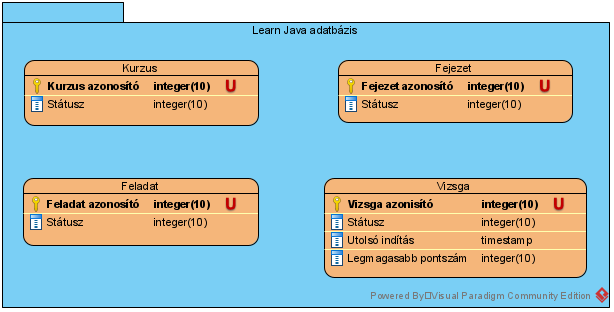
\includegraphics[width=\linewidth]{db_model}
	\end{center}
	
	Táblák közti kapcsolatra, külső kulcsokra nincs szükség. Az, hogy mely fejezetek és feladatok tartoznak egy-egy kurzushoz nem az adatbázisban van eltárolva, hanem a tananyagot definiáló \xml dokumentumokban (mivel nem változik dinamikusan).
	
	Az azonosítók megegyeznek az \xml dokumentumokban használt azonosítókkal. A státusz mezők mindig a fent definiált \textit{@Status} annotáció valamelyik értékét tartalmazzák.
	
	A vizsgák esetén vannak további dinamikusan változó adatok:
	
	\begin{itemize}
		\item Az utolsó indítás időpontja: Ez szükséges, hogy a \ref{vizsga} részben említett indítási korlátot be lehessen tartani.
		\item Legmagasabb pontszám: Dinamikusan változó, ezért az adatbázisban kell tárolni.
	\end{itemize}
	
	\subsubsection{Megvalósítás: SQLite és Room}\label{sqlite_roon}

	Az Android rendszer minden alkalmazás számára biztosít egy \textit{SQLite} relációs adatbázist. Számomra egyértelmű volt, hogy ezt fogom használni. Az \textit{SQLite} egy olyan adatbázis kezelő, amely nem kliens-szerver alapú, hanem közvetlenül az őt használó alkalmazásba van beágyazva. 
	
	Ennek előnye, hogy nem kell hálózati kapcsolat az adatbázis eléréséhez, és nem kell szervert üzemeltetni. Hátránya viszont, hogy minden adat lokálisan kerül eltárolásra. Ennél az alkalmazásnál ez nem jelent gondot, mivel viszonylag kevés rekord keletkezik (a tananyag minden eleméhez egy).
	
	Az alkalmazás saját adatbázisának közvetlenül is küldhetünk üzenetet, ez azonban több okból sem javasolt:
	
	\begin{itemize}
		\item Szintaktikus hibák: ha a kiadott \textit{SQL} utasításban szintaktikus hibát vétünk, az a program helytelen működéséhez, összeomlásához vezet. Ez nincs ellenőrizve.
		\item Érvénytelen utasítások: ha olyan utasítást adunk ki, amelyet az \textit{SQLite} nem tud végrehajtani, akkor is helytelen viselkedés fog történni. Például, ha olyan rekordot szúrunk be, ami sérti az egyediség feltételt.
		\item Adatbázis frissítés a főszálon: ha a főszálon adunk ki \textit{SQL} utasítást, akkor ez blokkolni fog, és a felhasználói felület nem lesz válaszképes. 
	\end{itemize}

	Pontos tervezéssel és helyes implementációval ez mind elkerülhető, de javasolt egy olyan keretrendszer használata, mely az adatbázis kezelés veszélyeit kezeli. Egy ilyen keretrendszer a \textit{Room}, amely az Android fejlesztői könyvtár (\textit{AndroidX}) része.
	
	A \textit{Room} elrejti a programozó elől az \textit{SQLite} adatbázist, helyette két komponenst biztosít, melyekkel a struktúrája és tartalma módosítható. Ezen kívül meg fogja tiltani, hogy a főszálról adatbázis műveletet végezzünk (ilyen esetben kivétel dobódik). 
	
	\subsubsection{Room entitások}
	
	Az entitások olyan \textit{@Entity} annotációval jelölt Java osztályok, melyek megadják az adatbázis tábláinak struktúráját. Például a fejezet táblát a következőképpen definiáltam:
	
	\begin{lstlisting}[language=Java]
@Entity(tableName = "chapter_status")
public class ChapterStatus {
	
 @PrimaryKey //külső kulcs jelző
 @ColumnInfo(name = "chapter_id")
 private int chapterId;
	
 @ColumnInfo(name = "status")
 @Status //saját státusz annotáció
 private int status;
 
 //konstruktor...
}
	\end{lstlisting}  
	
	Látható, hogy annotációk segítségével adhatjuk meg, hogy milyen mezői legyenek az adott táblának. Az alkalmazás indításakor ez a tábla létre fog jönni az adatbázisban, anélkül, hogy egyetlen \textit{SQL} utasítást is írnunk kellene. Azokat a \textit{Room} fogja összeállítani, az általunk megadott adatok alapján, és garantáltan helyesek lesznek.
	
	A későbbiekben ezt az osztályt példányosíthatjuk, ezek az objektumok rekordokat fognak reprezentálni.

	\subsubsection{Room adatkezelők}
	
	Az adatkezelő objektumok olyan \textit{@Dao} annotációval jelölt Java interfészek, amikkel az előző részben definiált táblák tartalmát módosíthatjuk. Például a fejezet táblához a következő módosító interfészt készítettem:
	
	\begin{lstlisting}[language=Java]
@Dao
public interface ChapterDao {
	
 @Insert //a beszúró SQL utasítás automatikusan generálódik
 void addChapterStatus(ChapterStatus chapterStatus);
	
 @Update //a frissítő SQL utasítás automatikusan generálódik
 void updateChapterStatus(ChapterStatus chapterStatus);
	
 @Query("SELECT * FROM chapter_status WHERE chapter_id == :chapterId")
 ChapterStatus queryChapterStatus(int chapterId);
}
	\end{lstlisting}

	Bizonyos egyszerű műveletekre vannak előre adott annotációk, melyek automatikusan fogják generálni a a megfelelő \textit{SQL} utasítást (beszúrás, frissítés, törlés). Ezek azonban nem elegendőek, ezért a \textit{@Query} annotációval saját utasítást írhatunk. Ennek a tartalma fordítási időben ellenőrizve lesz. Megfigyelhető, hogy még arra is lehetőség van, hogy a kapott paraméterek értékét behelyettesítsük az \textit{SQL} utasításba. A fenti kódban is látható egy saját utasítás, ami képes az adatbázisból egy fejezetet az azonosítója alapján lekérni.

	Ezután az adatbázist ezzel az interfésszel módosíthatjuk, anélkül, hogy a kód más részeibe \textit{SQL} utasítást kelleni írni. Ez növeli a karbantarthatóságot és 
	csökkenti az \textit{SQL} írásakor gyakran előforduló hibákat (elírt tábla vagy oszlop név). A következő kódminta például hozzáad egy új fejezetet az adatbázisba, ami elérhető lesz (\textit{UNLOCKED} státusz):
	
	\begin{lstlisting}[language=Java]
//egy új szálon
new Thread(() -> {
 ChapterDao dao = ... ;
 ChapterStatus cs = new ChapterStatus(id, Status.UNLOCKED);
 //beszúrás
 dao.addChapterStatus(cs);
}).start();
	\end{lstlisting}
	
	Itt nagyon fontos, hogy az adatbázis művelet új szálon fut és nem az alkalmazás főszálán. A főszálon futtatott hosszú művelet megakasztaná a program felhasználói felületét is, amitől az úgy tűnik, mintha "lefagyott" volna. Az Android újabb verziói esetén már maga a rendszer is tiltja, hogy ilyen műveleteket 
	a főszálon végezzünk, ezzel kényszerítve a programozókat reszponzív alkalmazások írására. Ez a korlátozás más típusú műveletekre is érvényben van, például hálózati operációt sem lehet főszálon végezni.
	
	Megjegyzem, hogy a fenti kódmintában az olvashatóság érdekében a háttérszálon történő futtatás egyszerű formában látható (\textit{Thread} osztály). Az alkalmazás kódjában ez összetettebb és hatékonyabb módon van megvalósítva. 
	
	\subsubsection{Megvalósítás: szerver alkalmazásban}
	
	Ahogy a tananyag tárolásával (\ref{tananyag_tarolasa}) kapcsolatban is felmerült a szerver használata, úgy itt is megjelenik, mint lehetőség. Az adatbázist kezelhetné a szerver, melyet az alkalmazás \textit{REST API} segítségével ér el. Ennek előnye, hogy az adatbázis biztonságosabbá válna. Míg az \textit{Android}-os eszközön lévő adatbázist a felhasználó el tudja érni és módosíthatja, addig a szerverhez nincs hozzáférése. Ez az előny azonban nem olyan jelentős, mivel ez az alkalmazás nem biztonság kritikus. 
	
	Hátrány, hogy a tananyagban történő előrehaladás mentése így internet kapcsolatot igényelne. Az adatbázis struktúrája is bonyolódna. A \ref{adatbazis_struktura}. fejezetben látható modell egy felhasználót ír le, ilyenből a szervernek többet is kezelnie kellene.
	
	A szerveroldali adatbázis nem merült fel valós lehetőségként, ugyan azon okok miatt, mint ahogy a tananyag tárolásához sem használtam a szervert.

	\subsection{Hirdetések az alkalmazásban}
	
	A fejlesztés során elkezdett érdekelni, hogy miként lehet hirdetéseket integrálni egy androidos alkalmazásba, ezért megvalósítottam ezt. Természetesen figyeltem arra, hogy a megjelenő hirdetések ne legyenek zavaróak és csak időnként jelenjenek meg.
	
	A hirdetések megjelenítéséhez a \textit{Google AdMob} saját androidos könyvtárat biztosít, amellyel megkönnyíti a fejlesztők dolgát. A programozónak annyi a dolga, hogy regisztrálja az alkalmazását az \textit{AdMob} oldalán, ahol hirdetési kulcsokat kap. Ezután pedig az alkalmazás képernyő elrendezéseibe be kell szúrni egy hirdetés nézetet, úgy, ahogy egy egyszerű gombot vagy szövegnézetet illesztenénk be. A könyvtár elrejti a következő nehézségeket:
	
	\begin{itemize}
		\item Hálózati műveletek: honnan és hogyan kell letölteni a hirdetést.
		\item Személyre szabás: milyen hirdetés jelenjen meg az adott felhasználónak.
		\item Megjelenítés: kép megjelenítése, videó lejátszása. Annak kezelése, hogy a felhasználó eltünteti a hirdetést.
	\end{itemize} 

	A fentiek figyelembe vételével a következő helyekre raktam hirdetéseket az alkalmazásban:
	
	\begin{itemize}
		\item Kurzus-, és fejezetválasztó képernyők: itt kis, úgynevezett \textit{banner} hirdetések jelennek meg.
		\item Fejezet vagy feladat \textbf{bezárásakor}: itt 50\% eséllyel jelenik meg egy egész képernyős, úgynevezett \textit{interstitial} hirdetés.
	\end{itemize}

	Az \textit{AdMob} által adott hirdetési kulcsok biztonsági szempontból kritikusak, ezért nem vittem fel őket a verziókövető rendszerbe sem, csak a saját fejlesztőkörnyezetemben vannak meg. 
	
	Fontos, hogy a valódi kulcsokat nem szabad használni a fejlesztés és tesztelés során, csakis a végleges, kiadott változatokban. Ennek oka, hogy az \textit{AdMob} el akarja kerülni, hogy a szervereit felesleges terhelés érje fejlesztés vagy tesztelés alatt álló alkalmazásoktól. A programozónak azonban mindenképpen meg kell győződnie arról, hogy az általa elhelyezett hirdetések megfelelően működnek (megjelenik-e? jó helyen jelenik-e meg?). Az ilyen esetekre az \textit{AdMob} teszt kulcsokat biztosít. Ezeket bármilyen céllal fel lehet használni, ilyenkor a valódi hirdetésekkel azonosan viselkedő, de teszt szövegeket megjelenítő "hirdetések" töltődnek be. Itt a kurzusokat listázó képernyő látszik, ahol betöltődött egy teszt hirdetés:  
	
	\begin{center}
		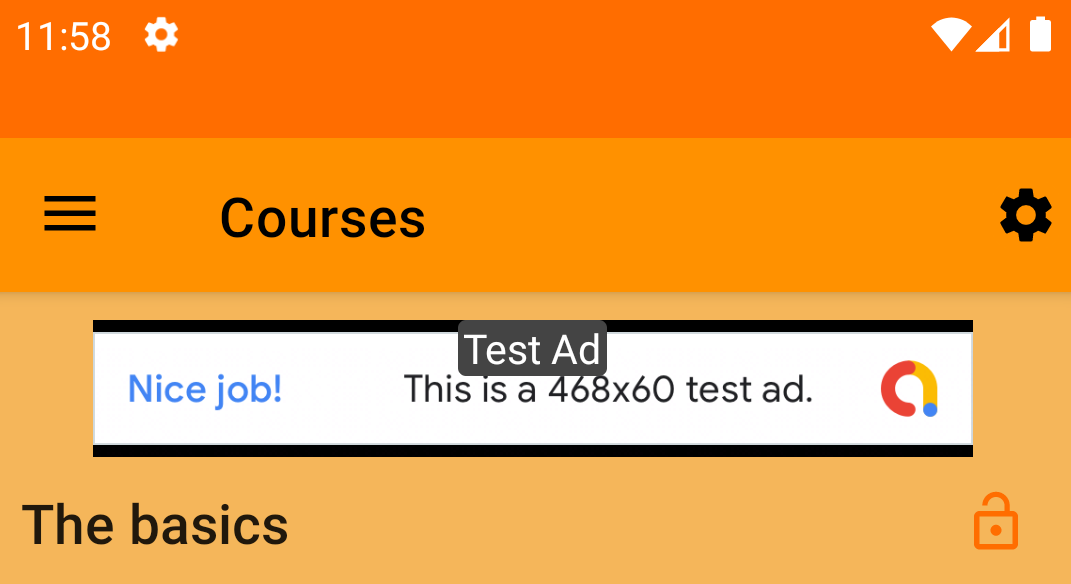
\includegraphics[width=5cm]{test_ad}
	\end{center}

	A hirdetési fiók tulajdonosa bevételhez jut, ha a felhasználók az éles hirdetések valamelyikére kattintanak. Megjegyzem, hogy mivel az alkalmazást eddig nagyon kevesen töltötték le, ezért az ebből származó bevételeim is igen csekélyek, havonta nagyjából 20-30 Forintot tesznek ki.

	\section{A ClipSync funkció}\label{clipsync}
	
	Az alkalmazás útmutatójában arra biztatom a felhasználót, hogy mindenképpen telepítsen fejlesztőkörnyezetet a számítógépére, ahol végigkövetheti a tananyagot (ehhez egy útmutatót is készítettem, ami a legelső fejezetben található). Ha valaki így használja az alkalmazást, annak nagyon hasznos lehet, ha a tananyagban lévő kódmintákat egyszerűen át tudja vinni a számítógépére, ahol azonnal beillesztheti őket fejlesztőkörnyezetbe.
	
	Rövid kutatás után kiderült, hogy ilyen funkcionalitást biztosító programok vannak, még \textit{Android}ra is és a legtöbb helyen \textit{ClipSync} (\textit{clipboard synchronization}, azaz vágólap szinkronizálás) néven szerepelnek. Az alkalmazás első verzióiban átirányítottam a 
	felhasználót egy ilyen tudással rendelkező alkalmazáshoz. A fejlesztés során azonban, több okból fakadóan, úgy döntöttem, hogy ezt a funkciót beépítem az alkalmazásba. Ezek az okok a következőek voltak:
	
	\begin{itemize}
		\item Úgy véltem, hogy a felhasználónak kényelmetlenséget okoz és nem ideális, ha az alkalmazás optimális használatához további alkalmazás letöltésére van szükség.
		\item Szerettem volna kipróbálni, hogy miként küldhetnek és fogadhatnak adatokat az alkalmazások \textit{Android}on, az eszköz \textit{Bluetooth} kapcsolata segítségével.
	\end{itemize} 
	
	Úgy határoztam, hogy két különböző módot is implementálok, amelyekkel meg lehet osztani a kódmintákat: egyet a \textit{Bluetooth} segítségével, a másikat pedig hálózaton keresztül. Az alkalmazás önmagában azonban egyikhez sem elég, mivel ez csak küldeni tudja az adatokat. Kellett egy program, ami a számítógépen fut és képes fogadni az érkező adatokat, majd azokat vágólapra másolni. Ezt \textit{ClipSync} szervernek neveztem el.
	
	\subsection{ClipSync szerver}
	
	A "szerver" program azon a számítógépen fut, ahová az alkalmazásban kiválasztott kódmintáknak kerülniük kell. Minimális felhasználói felülettel rendelkezik, amit a \textit{Java Swing} keretrendszerrel készítettem el, így platform független. Ahogy az alkalmazás, úgy ez is rendelkezik magyar és angol változattal is.
	
	\begin{figure}[h!]
		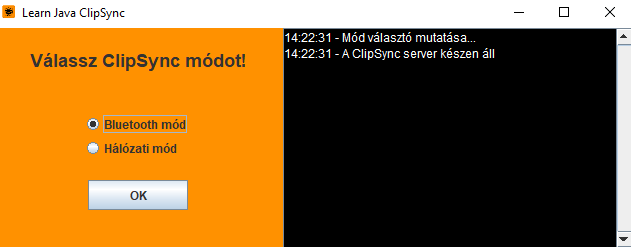
\includegraphics[width=6cm]{clipsync_server_select}\hfill
		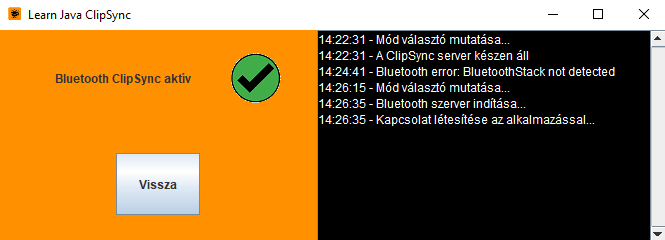
\includegraphics[width=6cm]{clipsync_server_bluetooth}
		\caption{A mód választó és a \textit{Bluetooth} képernyők, a szerver magyar változatából.}
	\end{figure}

	Természetesen előfordulhat, hogy a futtató számítógép nem alkalmas az adatok fogadására valamelyik módon (például nem rendelkezik \textit{Bluetooth}-al). Ilyenkor hibaüzenet jelenik meg.
	
	\begin{figure}[h!]
		\centering
		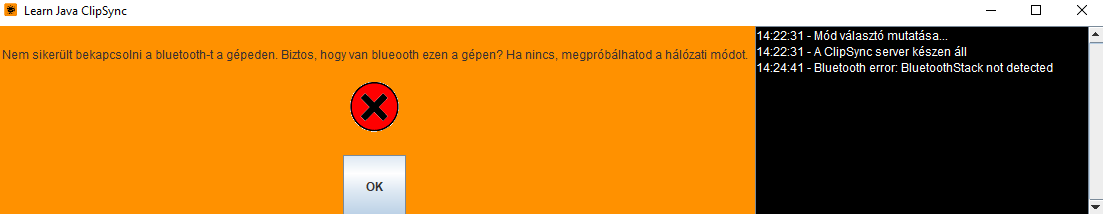
\includegraphics[width=10cm]{clipsync_server_error}
		\caption{\textit{Bluetooth} hiba képernyő, a szerver magyar változatából.}
	\end{figure}
	
	A szerver letöltési linkjét megjelenítettem az alkalmazáson belül, ahogyan az utasításokat is a beüzemelésére. Ezek megtalálhatóak a szerver weboldalán, ami \textit{GitHub} segítségével van hostolva és a \ref{qr_clipsync}. ábrán látható \textit{QR} kóddal érhető el.

	\begin{figure}[h!]
		\centering
		
\includegraphics[width=5cm]{clipsync_server_qr}
		\caption[ClipSync szerver caption.]{\textit{QR} kód, amivel elérhető a ClipSync szerver oldala. Ha a kód nem működne, lásd a lábjegyzetet\footnotemark.}
		\label{qr_clipsync}
	\end{figure}
	\footnotetext{A ClipSync szerver linkje: \url{https://github.com/Gtomika/learn-java-clipsync}}

	A felhasználó, érthető módon, vonakodhat attól, hogy számára ismeretlen forrásból letöltött programokat futtasson. Annak igazolására, hogy a program semmilyen káros kódot nem tartalmaz, nyílt forráskódúvá tettem. A forráskód szintén a fenti linkről érhető el.
	
	\subsection{Bluetooth mód}
	
	Az első lehetőség a kódminták megosztására a \textit{Bluetooth}. Ennek használhatóságához több feltételnek is teljesülnie kell:
	
	\begin{itemize}
		\item Mind az androidos eszköz, mind a számítógép rendelkezik \textit{Bluetooth}-al.
		\item A felhasználó megadja a szükséges engedélyeket (ezek az \textit{Android} verziójától függően változnak).
	\end{itemize}

	Ha ezek teljesülnek, akkor elindulhat a párosítási folyamat, ami az alkalmazáson belülről levezényelhető. Természetesen, ha a két eszköz már korábban párosításra 
	került, akkor erre a lépésre nincs szükség.
	
	Amint a két eszköz párosítva van, és a felhasználó kiválasztotta a \textit{Bluetooth} módot mind az alkalmazáson, mind a \textit{ClipSync} szerveren belül, a kódminták mellett lévő másolás gombok küldik a minta tartalmát.
	
	\subsection{Hálózati mód}
	
	Ezt a módot alternatívaként vezettem be azoknak, akik nem kívánnak végigmenni a nehézkes \textit{Bluetooth} párosításon, vagy nem áll rendelkezésükre \textit{Bluetooth} valamelyik eszközön. A következő feltételek mellett használható:
	
	\begin{itemize}
		\item Az androidos eszköz és a számítógép ugyanazon a helyi hálózaton vannak.
		\item Az androidos eszköz \textbf{nem mobil HotSpot}, azaz nem osztja meg a saját internetét.
	\end{itemize}

	A megvalósítás igen egyszerű, az alkalmazás szórt üzenetet (\textit{broadcast}-ot) küld a helyi hálózatra, amit a szerver figyel. Ha olyan adatot kap, ami az alkalmazástól jött, akkor arra válaszol. Az alkalmazás attól függően értesíti a felhasználót, hogy ez a válasz megjött-e.  
	
	\section{A játszótér funkció}\label{playground}

	Mivel az alkalmazás a programozásról szól, szerettem volna egy olyan lehetőséget beépíteni, ahol a felhasználó az alkalmazáson belül készíthet egyszerűbb Java programokat, és azokat futtatni is tudja. Ennek a \textit{játszótér} nevet adtam (angol változatban \textit{playground}). Már az elejétől fogva tudtam, hogy ez jelentős feladat lesz, ahol nehézséget főleg ez a két dolog fogja okozni:
	
	\begin{itemize}
		\item Dinamikusan szerkeszthető kódminta, ami formázottan jelenik meg.
		\item A kód futtatása, és a kimenet, vagy a hibák megjelenítése.
	\end{itemize}

	\subsection{Dinamikusan formázott kód}\label{dinamikusan_formazott_kod}
	
	A célom az volt, hogy olyan kódot jelenítsek meg, ami kinézetében megegyezik a fejezetekben és feladatokban látható statikus kódmintákkal (\ref{kodmintak}), és az úgynevezett interaktív kódmintákkal (\ref{interaktiv_kodmintak}), de teljes mértékben szerkeszthető.  
	
	A \ref{kodmintak}. fejezetben leírtam, hogy a tananyagban lévő kódmintákat egy erre célra készült, főleg reguláris kifejezéseket használó program segítségével formáztam meg, majd a tananyagot alkotó \xml fájlokba már a formázott kód került. Ez a megközelítés nem kivitelezhető a játszótér esetén, mert a lehetséges kódminták száma végtelen.
	
	A probléma megoldására a már meglévő formázó programot használtam, amit kisebb módosításokkal beépítettem az alkalmazásba. Ezt nagyban segítette, hogy mind az alkalmazás, mind a formázó program azonos nyelven, Java-ban íródtak. A kód formázása így már dinamikusan megoldható, és minden esetben újra fog futni, ha a felhasználó szerkeszti a tartalmát. Ezt persze optimalizálásnak vetettem alá, mivel a formázás viszonylag hosszú folyamat. Az alkalmazás megvárja, amíg a felhasználó már nem gépel, és csak utána indít formázást.
	
	A \ref{playground_code_figure}. ábra mutatja a szerkesztőfelületet. Ahogy a képen is látszik, több forrásfájl is támogatott, ezek közül mindig a kiválasztott jelenik meg.
	
	\begin{figure}[h!]
		\centering
		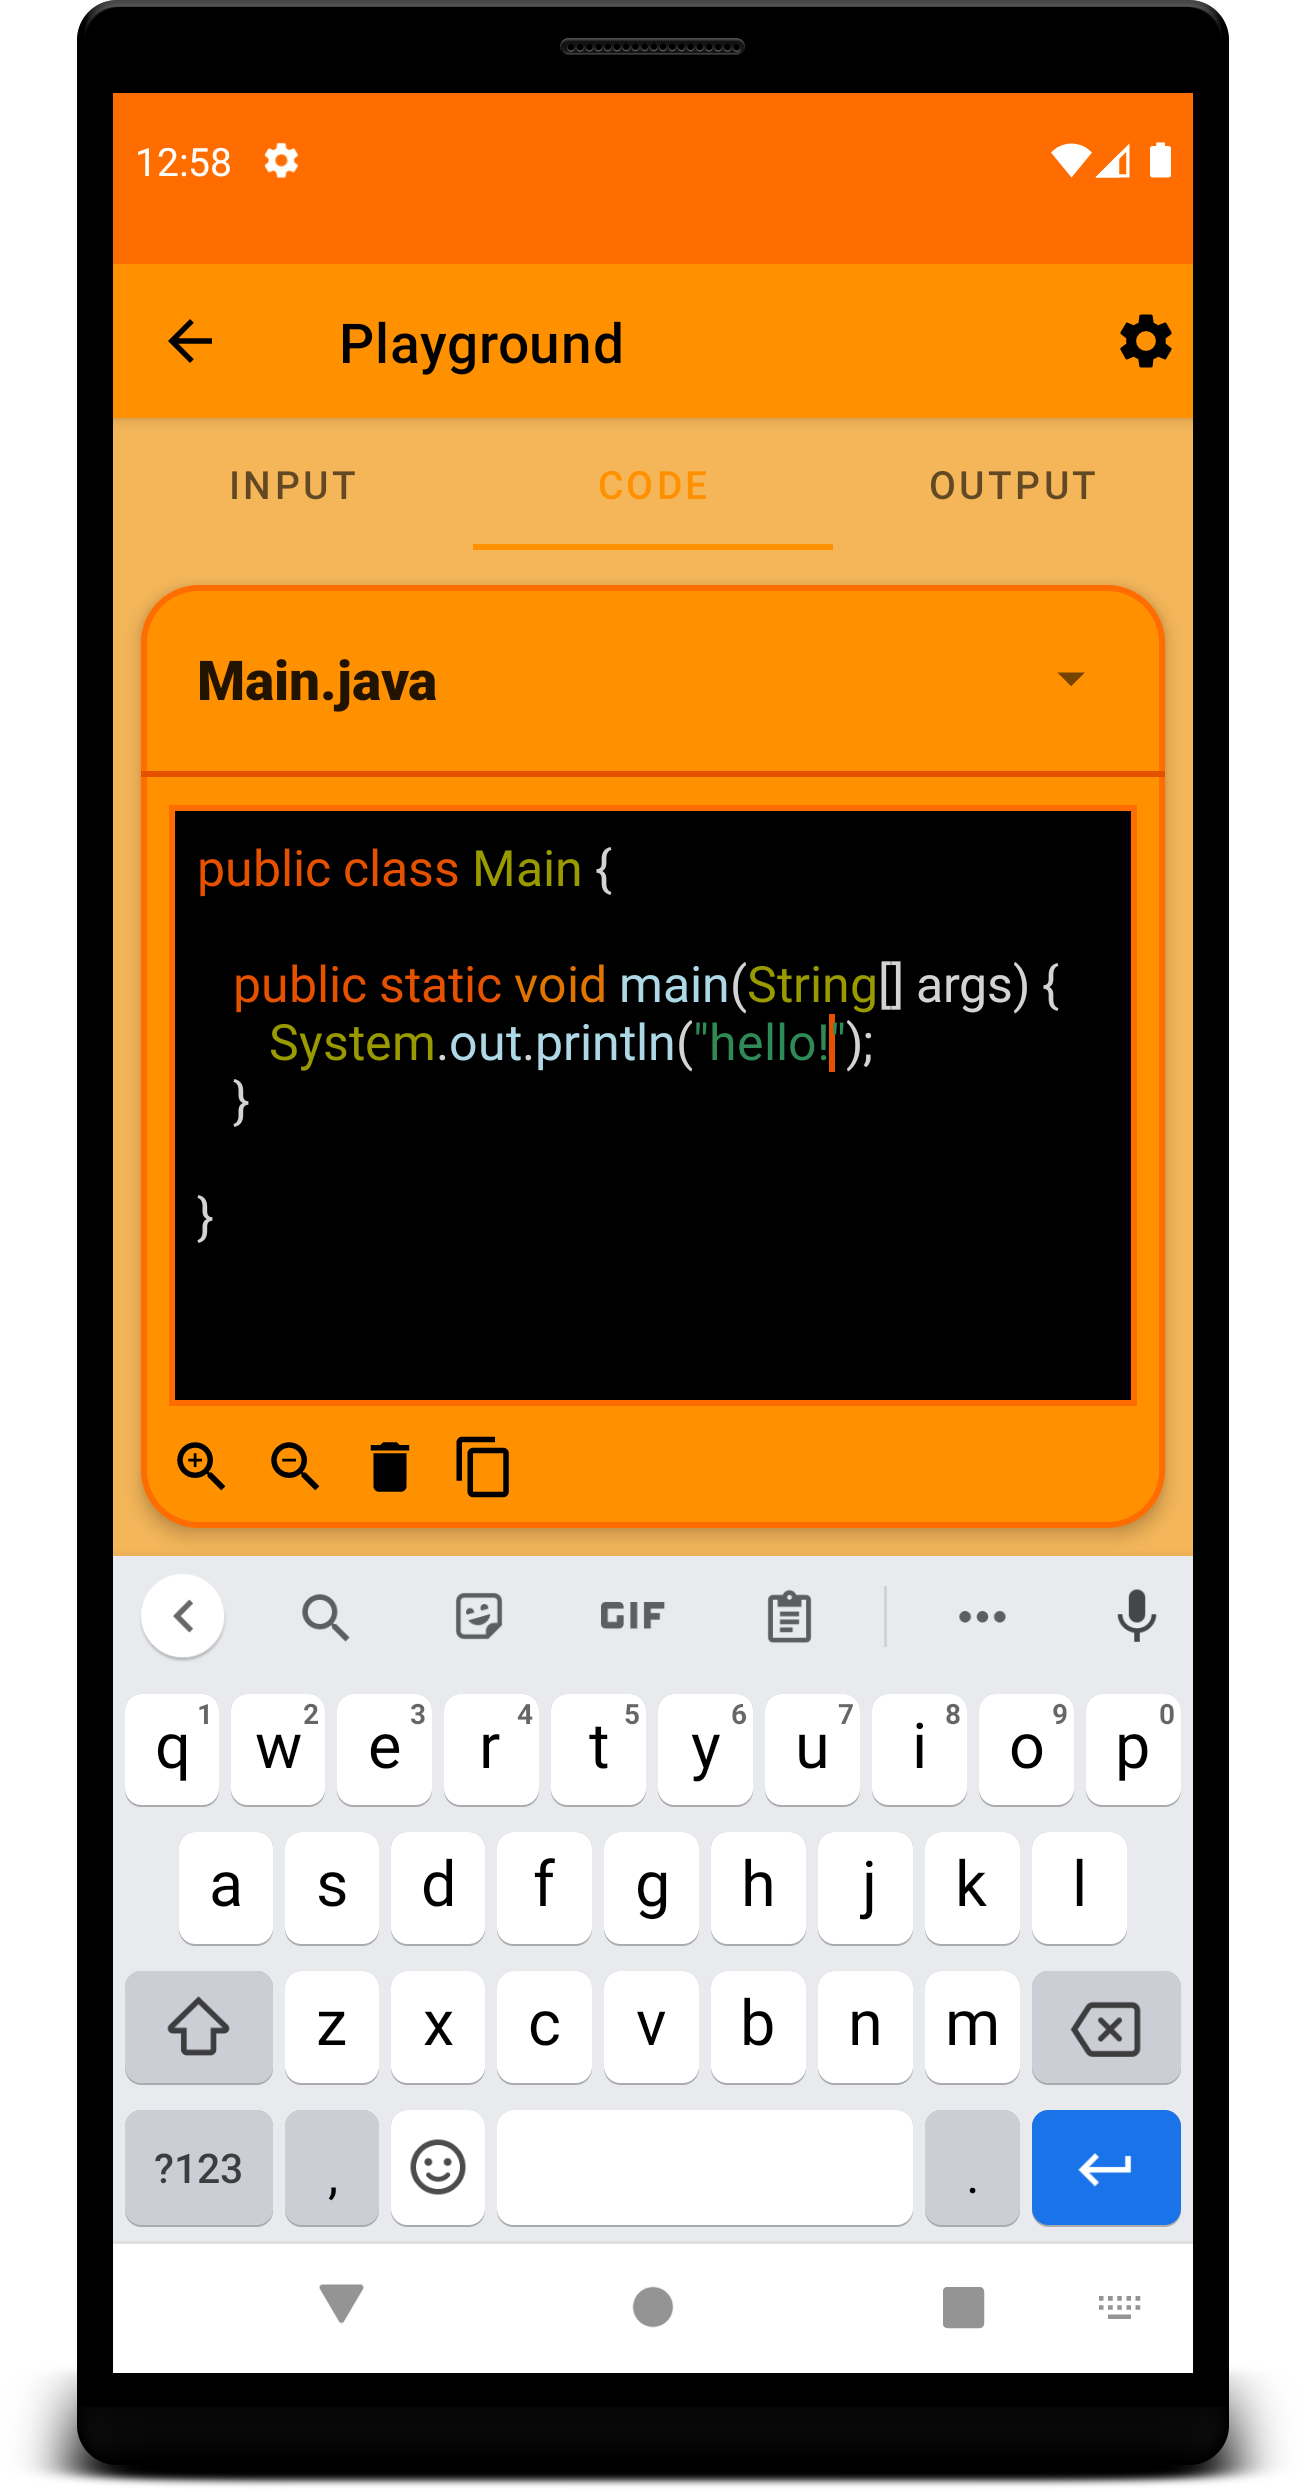
\includegraphics[width=5cm]{playground_code}
		\caption{Kód szerkesztése az alkalmazás angol változatában.}
		\label{playground_code_figure}
	\end{figure}

	Ahhoz, hogy az induláskor ne kelljen túl sokat gépelni, sablonokat készítettem. Például a \textit{Main.java} "fájl" alapból tartalmazni fogja az osztály deklarációt, és azon belül a főmetódust. Az alkalmazás menti a megírt kódot, és az a játszótér újbóli megnyitása esetén be fog töltődni. 

	\subsection{Futtatás}
	
	Több lehetőséget is számba vettem, hogy miként lehetne a megírt kódot lefuttatni.
	
	\begin{enumerate}
		\item Futtatás helyben, az \textit{Android} eszközön.
		\item Szerver alkalmazás készítése, ami megkapja a kódot és futtatja, majd az eredményt visszaküldi.
		\item Már létező \textit{API} használata.
	\end{enumerate}

	Először az első lehetőséget szerettem volna megvalósítani, mivel ez nem igényel internetkapcsolatot és költségekkel sem jár, mert nem kell szervert fenntartani, vagy fizetni bármilyen \textit{API} használatáért. Ezt azonban nem tudtam megvalósítani. Több fórumon való konzultáció után kiderült, hogy az általános vélekedés szerint lehetetlen Java kódot fordítani és futtatni Android eszközön. Találtam ugyan olyan alkalmazást a \textit{Play} áruházban, ami képes erre, de nem tudtam megfejteni, hogy hogyan működik.
	
	Ezután saját szerver alkalmazásban gondolkodtam. \textit{Spring Boot} alapú szervert szerettem volna, mivel ez Java-ban íródik és a Java viszonylag jó felületet biztosít fordításra és futtatásra, a \href{https://docs.oracle.com/javase/7/docs/api/java/lang/Compiler.html}{\textit{java.lang.Compiler}} segítségével (ez sajnos Android-on nem csinál semmit). Kiderült azonban, hogy ilyen szerver készítése nehezebb, mint vártam. Ki kell dolgozni, hogy hol hozza létre a kapott forrásfájlokat, úgy, hogy akár egyszerre több futtatási kérés is érkezhet. 
	
	Továbbá komoly biztonsági kockázat is van, ugyanis a felhasználó lényegében bármilyen kódot küldhet, ami aztán a szerveren fut majd. Ennek kivédésére a \href{https://docs.oracle.com/javase/8/docs/api/java/lang/SecurityManager.html}{\textit{java.lang.SecurityManager}} osztály használatát terveztem, amivel meg lehet akadályozni a fájl írást vagy a hálózati hívásokat.
	
	A saját szerver tervezése közben felmerült sok nehézség miatt úgy döntöttem, hogy már létező \textit{API}-t keresek, ami tud Java fordítást és futtatást készíteni.
	Meglepetésemre találtam olyan ingyenes és nyílt forráskódú futtató \textit{API}-t, ez a \href{https://glot.io/}{\textit{Glot.io}}\footnote{A Glot.io itt érhető el: https://glot.io/}. A dolgozat írásakor az alkalmazás ezt használja a futtatásra, azonban a jövőben ez lehet, hogy megváltozik. A \textit{Glot.io}-nál ugyan nincsenek időbeli vagy mennyiségi korlátok, de elképzelhető, hogy tiltana, ha túl sok hívás érkezik az alkalmazástól.
	
	Megjegyzem, hogy a \textit{Glot.io} a saját szerver legtöbb problémáját elegáns módon, \textit{Docker} konténerek használatával hidalja át. A jövőben, ha mégis saját szerver mellett döntök, én is ezt a módszert fogom alkalmazni.

	\begin{figure}[h!]
		\centering
		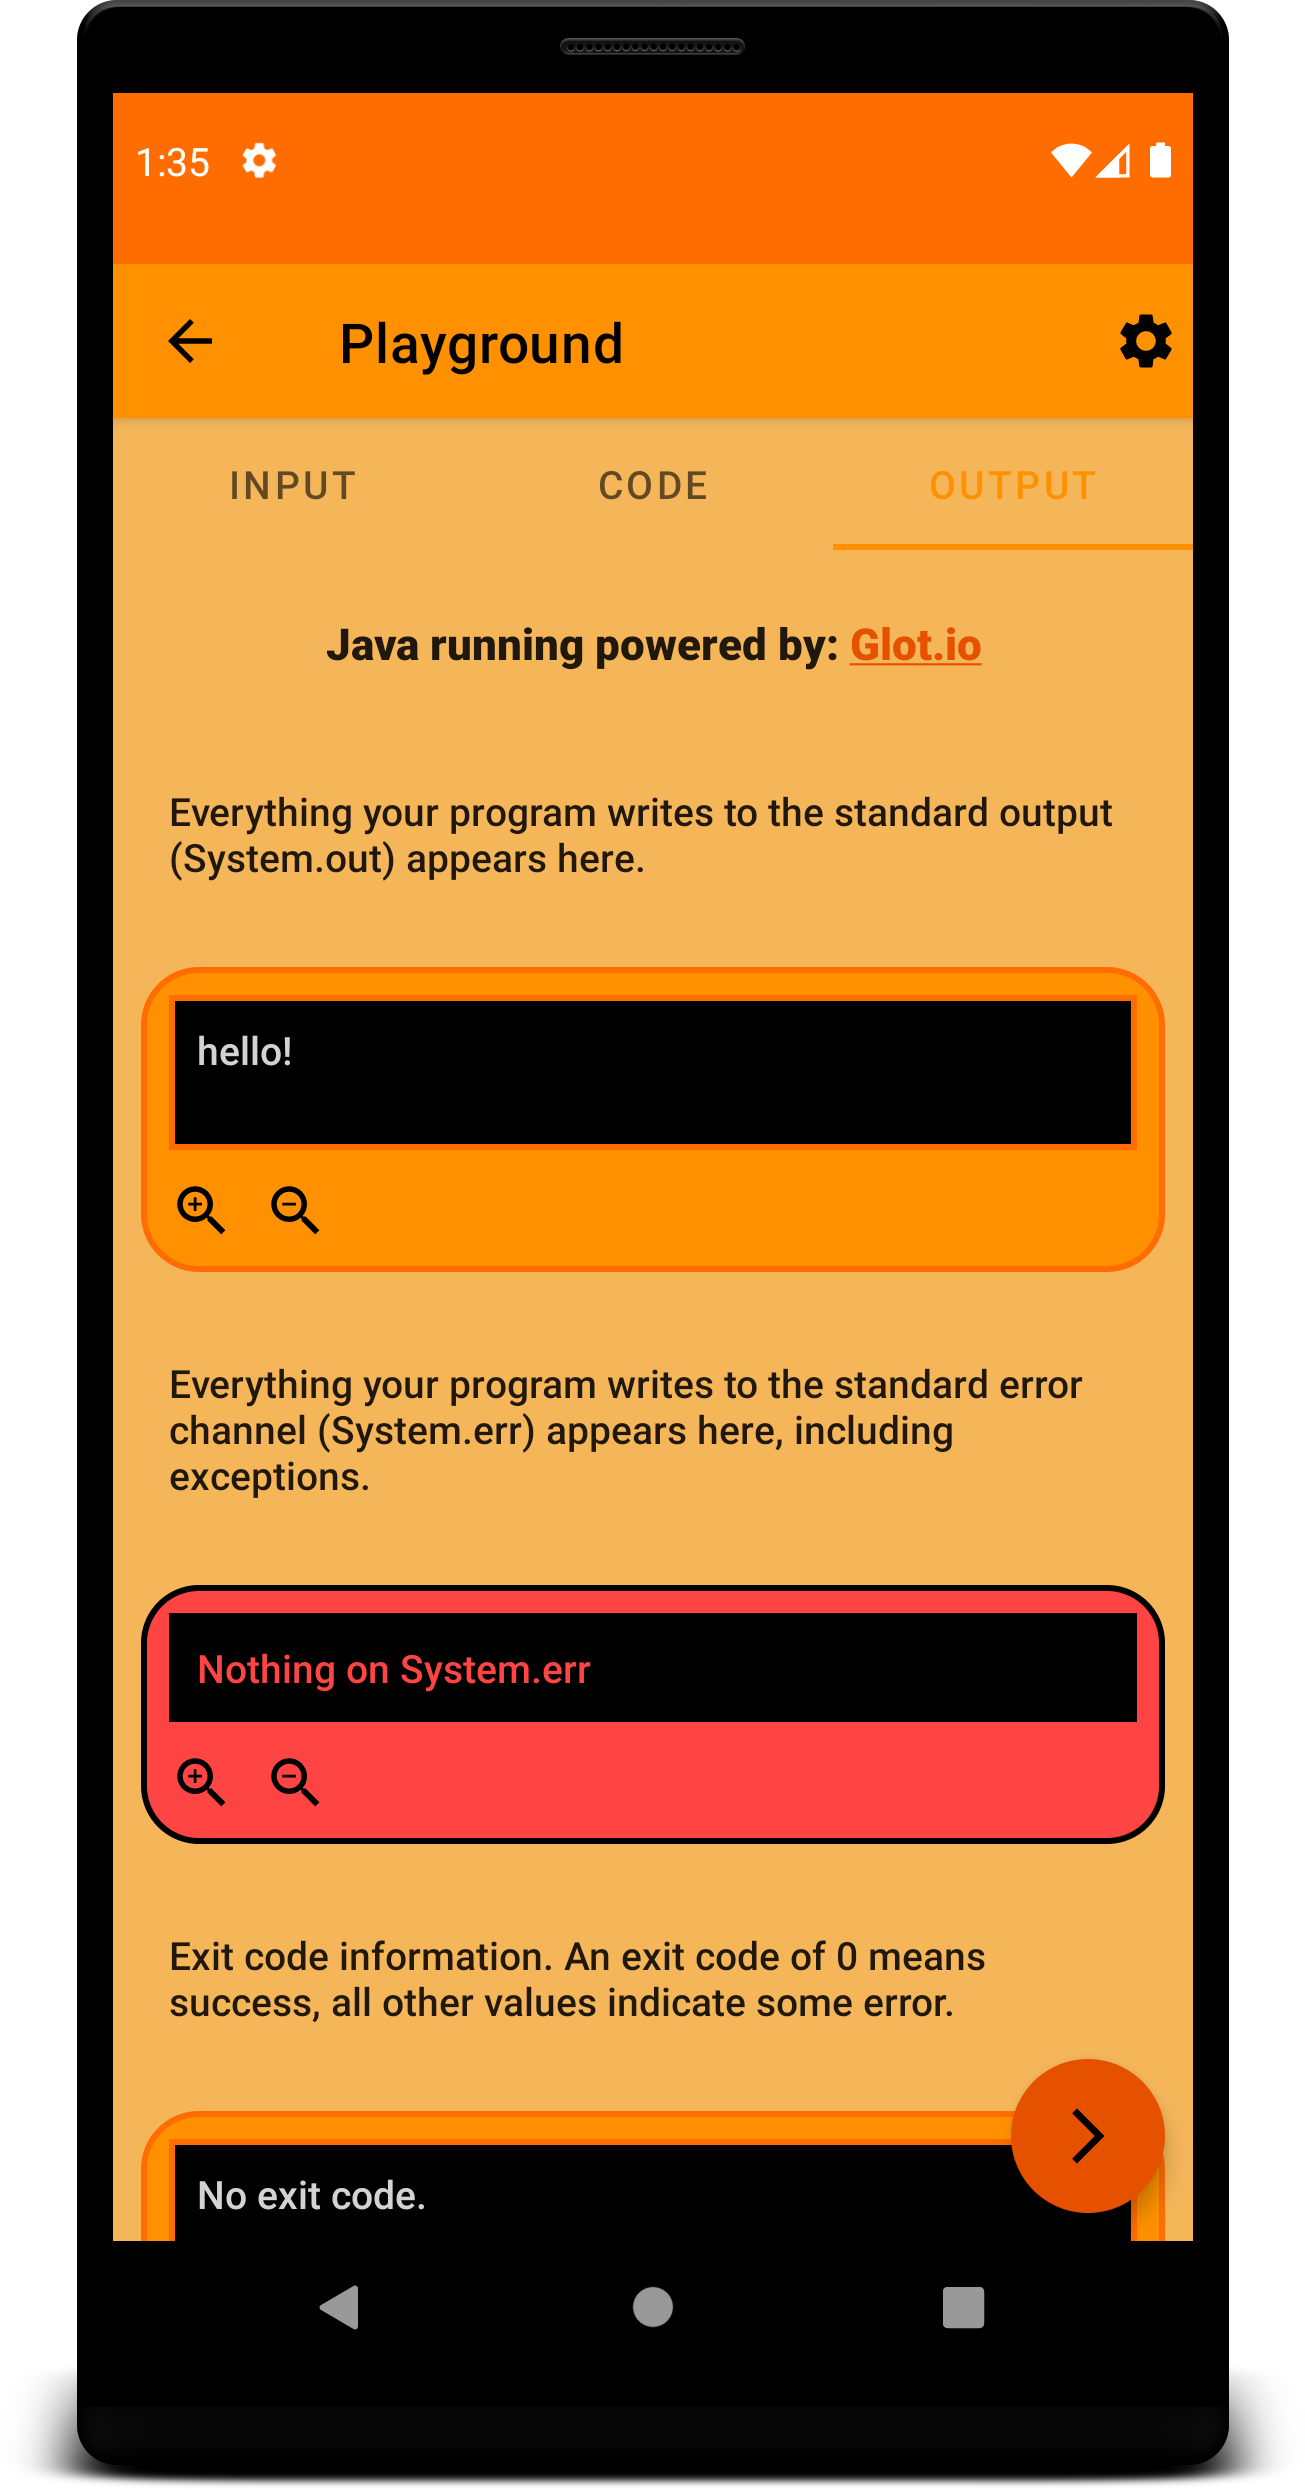
\includegraphics[width=5cm]{playground_output}
		\caption{Az eredményablak, miután futtattuk a \ref{playground_code_figure}. ábrán látható kódot.}
		\label{playground_output_figure}
	\end{figure}

	A \ref{playground_output_figure}. ábrán látható a futtatás eredménye. Bemenet megadására is lehetőség van, ami standard inputra (\textit{System.in}) fog kerülni, ez a \ref{playground_code_figure}. és a \ref{playground_output_figure}. ábrák bal felső sarkában látható \textit{Input} rész kiválasztásával tehető meg.

	\section{Tesztelés}

	A tesztelés minden komoly szoftver fejlesztési folyamatának része. A teszteknek sok fajtája van, ezeket érdemes módszeresen végezni. 
	
	Az Android alkalmazások tesztelése jellemzően két teszt típussal történik, ezek az egységtesztek és az instrumentális tesztek. A továbbiakban részletesen írok ezekről és hogy az alkalmazás mely részeit teszteltem velük. 

	\subsection{Egységtesztek}
	
	Az egységtesztelés olyan alacsony szintű, fehérdobozos módszer, amellyel jellemzően a kód egy kis egységei, például metódusok tesztelhetőek. Majdnem minden tesztelési folyamatnak a részei, általában ezekből van a legtöbb egy tesztbázisban.  
	
	Az egységteszt mindig elszigetelten fut, a keretrendszer csakis azt a metódust fogja futtatni, amire az adott teszt vonatkozik, majd az eredményt ellenőrzi. Az ellenőrzés feltételekkel (\textit{assertion}) történik, például változókra és logikai kifejezésekre adhatunk meg feltételeket.
	
	Android esetén az egységtesztek a fejlesztő számítógépén futnak, nem pedig a mobil eszközön, vagy emulátoron. Ez lényegében azt jelenti, hogy tisztán \textit{Java} kódot tesztelhetünk, de olyat ami az Android fejlesztőcsomagból tartalmaz hívásokat már nem. Ebből következik, hogy az alkalmazáshoz sem férünk hozzá tesztelés közben.
	
	Ez jelentős limitáció, de azért egy Android alkalmazásnak is vannak olyan részei, amely tisztán \textit{Java} kódot tartalmaznak és ezek tesztelésére az egységtesztek a legalkalmasabbak. A dolgozat témáját alkotó alkalmazás tesztelésekor is használtam egységteszteket, azonban elég keveset, ennek oka éppen a fent említett korlát. Az általam kigondolt tesztesetek nagy részéhez ugyanis szükség van a futó alkalmazásra.
	
	A kód formázásának tesztelésekor például jól tudtam alkalmazni az egységteszteket. Ahogy azt a \ref{kodmintak}. és a \ref{dinamikusan_formazott_kod}. fejezetekben kifejtettem, az alkalmazás képes a kódminták formázott megjelenítésére. A formázást végző kód reguláris kifejezéseken alapul, nem használ semmit az Android fejlesztőcsomagból ezért egységtesztekkel is tesztelhető.
	
	Vegyük például a következő egyszerű utasítást, amit formázni szeretnénk:
	
	\begin{lstlisting}[language=Java]
String s;
	\end{lstlisting}
	
	A \ref{kodmintak}. fejezetben megadott formázási szabályok alapján itt egyedül a \textit{String} osztálynévnek kell kijelölést kapnia, ezért a formázott kódnak a következőképpen kell kinéznie (a konkrét színértéket az egyszerűség kedvéért nem mutatom):
	
	\begin{lstlisting}[language=Java]
<font color=...>String</font> s;
	\end{lstlisting}
	
	Ha tehát ismerjük az eredeti és a formázott kódot, ebből egyszerűen kapunk egy tesztesetet, ami egységtesztként megvalósítható (a \textit{Java} kód egységteszteléséhez általában használt \textit{JUnit} keretrendszerrel):
	
	\begin{lstlisting}[language=Java]
@Test
public void testClassFormatting() {
  String unformatted = "String s;";
  String formatted = formatter.formatContent(unformatted);
  assertEquals("...", formatted);
}
	\end{lstlisting}
	
	Az \textit{assertEquals} egyenlőség feltételt definiál, az első paraméter természetesen az elvárt, helyesen formázott kód, ami a formázó által adott eredménnyel lesz összehasonlítva (második paraméter).
	
	\subsection{Instrumentális tesztek}\label{instrumental_tests}

	Az instrumentális tesztek adják a megoldást az egységtesztek korlátjaira. Egy instrumentális teszt lényegében "egységteszt", de fontos különbség, hogy ezek Android eszközön (vagy emulátoron) futnak, és a keretrendszer minden teszt előtt elindítja az alkalmazásunkat. Ennek eredményeképpen itt már teljes körűen tesztelhetjük az alkalmazást, hozzáférünk az Android fejlesztő csomag osztályaihoz és az operációs rendszerhez is intézhetünk hívásokat.
	
	Az instrumentális tesztek futtatása is a \textit{JUnit} feladata, de ez önmagában nem elég, még két teszt keretrendszerre is szükség van:
	
	\begin{itemize}
		\item \textit{Espresso}: képes minden teszteset előtt a megfelelő helyen elindítani az alkalmazást (majd utána bezárni). A felhasználói felületére is hatni lehet vele, feltételeket lehet megfogalmazni a felület állapotára (lásd \ref{felhasznaloi_fel_teszt}).
		\item \textit{UI Automator}: nem az alkalmazást, hanem más alkalmazásokat és az Android rendszert irányíthatjuk és ellenőrizhetjük vele tesztek közben. Akkor hasznos, ha egy teszteset eredménye nem az alkalmazáson belül van (például azt szeretnénk tesztelni, hogy megjelent-e egy értesítés).
	\end{itemize}
	
	Az instrumentális teszt lehet fehérdobozos és feketedobozos is. Előbbire itt fogok példát adni, az utóbbira pedig a \ref{felhasznaloi_fel_teszt}. fejezetben.
	
	Ahhoz, hogy az itt következő tesztesetet az olvasó teljes mértékben megértse, pár mondatot írnom kell bizonyos Androidos koncepciókról. Az első az alkalmazáshoz tartozó \textit{preferenciák} fogalma. Ez egyszerű kulcs-érték párokat jelent, lényegében egy szótár adatstruktúra, ahol a kulcsok szövegek, az értékek pedig akármilyen primitív típusok lehetnek. Egy ilyen (kezdetben üres) preferencia szótár minden alkalmazásnak biztosított. Azok a kulcs-érték párok, amiket az alkalmazás ebbe belerak megmaradnak az újraindítások között is.
	
	Fejlesztésnél gyakori követelmény, hogy tudjuk, mikor indul először az alkalmazás. Ilyenkor általában különféle inicializálásokat kell elvégezni. Ezt a preferenciák segítségével a legegyszerűbb megoldani. Definiálunk egy kulcsot, például \textit{FIRST\_START} néven. Az alkalmazás minden induláskor megnézi, hogy ez a kulcs benne van-e a preferenciákban.  Ha még nincs, akkor tudjuk, hogy most indul először, futtathatjuk az inicializáló kódot, majd végül beletesszük a kulcsot a preferenciák közé. Ha a kulcs már jelen van, akkor az alkalmazás már nem az első alkalommal indul.
	
	Ezt a módszert én is használtam, a működését pedig egy instrumentális teszt segítségével ellenőriztem. A teszt elindítja az alkalmazást, majd pedig egy feltételt fogalmaz meg arra, hogy a preferenciák már tartalmazzák az első indítást jelölő kulcsot. Látható, hogy ez fehérdobozos teszt, mivel ismernünk kell hozzá a forráskódban lévő első indítás kulcs nevét. A teszt kódja (vázlatosan) itt látható:
	
	\begin{lstlisting}[language=Java]
@Test
public void testFirstStartPreference() {
  //preferenciák megszerése a 'prefs' változóba
  ...
  //feltétel a kulcs meglétére
  assertTrue(prefs.contains("FIRST_START"));
}
	\end{lstlisting}
	
	A fent említett \textit{Espresso} keretrendszer fog arról gondoskodni, hogy a teszteset előtt elindul az alkalmazás. Látható, hogy a feltétel megadásához itt még a \textit{JUnit} is elegendő. 
	
	\subsection{Felhasználói felület tesztek}\label{felhasznaloi_fel_teszt}
	
	A felhasználói felület (\textit{UI}) tesztek olyan instrumentális tesztek, ahol az alkalmazással kizárólag a felhasználói felület segítségével kommunikálunk, és a teszteset helyességét is a felület állapota adja meg. Ezzel nagyon jól lehet felhasználói interakciókat tesztelni, olyanokat mint "ha a felhasználó megnyomja az $X$ gombot, jelenjen meg az $Y$ szöveg". Ezek alapvetően feketedobozos tesztek, mivel az alkalmazással csakis a felhasználói felület segítségével beszélhetünk, mintha egy felhasználó használná. Ennek ellenére fehérdobozos elemek is vannak benne, mert a felület elemeinek beazonosításához általában a forráskódban definiált azonosítókat használunk.
	
	Az ilyen tesztek írásához már erősen ki kell használni az \textit{Espresso} által nyújtott lehetőségeket. Most példaként bemutatok néhány ilyen tesztet, melyeket az alkalmazás tesztbázisából vettem ki. Az első példa a vizsga képernyőhöz tartozik. Ezen a képernyőn van egy "befejezés" gomb, amivel a felhasználó lezárhatja a vizsgát (ennek a gombnak az azonosítója \textit{finish\_button}). Előtte azonban megjelenik egy megerősítő dialógus ablak, ami megkérdezi a felhasználótól, hogy biztosan befejezi-e a kitöltést. A megjelenő szövegkonstans neve \textit{confirm\_finish\_exam}. Ismerve az elvárt viselkedést, erre felhasználói felület tesztet írhatunk. A keretrendszer fog arról gondoskodni, hogy a teszt futása előtt megnyílik az alkalmazás megfelelő része (jelen esetben a vizsga képernyő).
	
	\begin{lstlisting}[language=Java]
@Test
public void testConfirmDialog() {
  //a befejező gomb megnyomása
  onView(withId(R.id.finish_button)).perform(click());
  //felétel arra, hogy látszik elem a megerősítő szöveggel
  onView(withText(R.string.confirm_finish_exam))
  	.check(matches(isDisplayed()));
}
	\end{lstlisting}
	
	Ebből a tesztesetből az \textit{Espresso} által nyújtott lehetőségek is jól látszanak. Be tudunk azonosítani egy elemet (vagy egyszerre többet) a felhasználói felületről, az azonosítója (\textit{withId}), az általa megjelenített szöveg (\textit{withText}) és még sok más alapján is.
	
	Amikor megvan az elem, akkor azon műveletet végezhetünk (\textit{perform}), ebben a tesztesetben például egy kattintást szimuláltam a vizsga befejező gombon. Továbbá beazonosított elemre feltételt is definiálhatunk (\textit{matches}). Ebben a tesztesetben az \textit{isDisplayed} feltételt tettem, ami akkor teljesül, ha az elem éppen megjelenik a képernyőn. Természetesen az itt látottakon kívül az \textit{Espresso} még sokféle műveletet és feltételt definiál.
	
	Érdemes egy-egy teszteset rendelni a felhasználó minden egyes döntéséhez. A fenti példához két döntés kapcsolódik: a felhasználó a megerősíti, hogy befejezi a vizsgát, vagy visszakozik. Ezt a két döntést a megjelenő dialógusablak megfelelő gombjainak megnyomásával (szintén a \textit{perform} segítségével) lehet szimulálni. Ezeket a teszteseteket meg is valósítottam, és a vizsga eredményét megjelenítő nézetre tettem feltételt. Ha felhasználó megerősíti, a befejezést, akkor a feltétel az, hogy ez a nézet látszódik (\textit{isDisplayed}), ha pedig visszakozik, akkor az elvárt viselkedés, hogy az eredménynézet nem jelenik meg (erre is van beépített feltétel, \textit{isNotDisplayed}).
	
	Az eddig bemutatott instrumentális tesztek az egyszerűbbek közé tartoznak. A gyakorlatban a tesztek általában több felhasználói interakció szimulálásából, és több feltétel megadásából állnak. Ilyen összetett teszt például az, amit a vizsga folyamat teljes ellenőrzésére készíttettem. Ez a teszt megnyit egy próba vizsgát, ami minden kérdéstípusból tartalmaz néhányat, fix sorrendben. Az \textit{Espresso} keretrendszer segítségével a tesztet úgy programoztam, hogy az összes kérdésre adja meg a helyes választ, majd zárja le a vizsgát. A folyamat során több feltételt is ellenőrzök, például, hogy sikeresen befejeződött-e a vizsga, és hogy maximális pontszám lett-e megadva. A teszt futásáról videót is készítettem, ahol látszik, hogy a keretrendszer emberfeletti sebességgel kitölti a próbavizsgát, majd megkapja rá a legmagasabb pontszámot. A videóért lásd a \ref{qr_instrumental_test}. ábrát.
	
	\begin{figure}[h!]
		\centering
		
\includegraphics[width=5cm]{instrumental_test_qr_code}
		\caption[Alkalmazás instrumentális teszt Caption]{\textit{QR} kód, amivel megnézhető egy instrumentális teszt. Ha a kód nem működne, lásd a lábjegyzetet\footnotemark.}
		\label{qr_instrumental_test}
	\end{figure}
	\footnotetext{Az instrumentális teszt videó linkje: \url{https://youtu.be/4YkI0qD0FVg}}
	
	 Az instrumentális tesztek egyik alapelve, hogy ne rendelkezzenek külső függőséggel. Külső függőségről akkor beszélünk, ha például a teszteset hívást intéz egy szerver felé, és a sikerhez a szerver válaszára is szükség van. Ilyen tesztek esetén az ajánlás az, hogy szimuláljuk (\textit{mock}-oljuk) a külső függőséget úgy, hogy a válasz biztos megérkezik. Ehhez az ajánláshoz én is igyekeztem tartani magamat a tesztek írása közben. Például azoknál a teszteseteknél, amiknek része volt kód futtatása (játszótér funkció, lásd \ref{playground}.) a külső \textit{API} hívásokat helyettesítettem olyanokkal, amik mindig válaszolnak. 
	 
	 Ennek ellenére néhány esetben nem tudtam elkerülni a külső függőséget. Ilyek voltak például azok a tesztek, amikkel az alkalmazás és \textit{ClipSync} szerver (lásd \ref{clipsync}) együttműködését ellenőriztem. Ezek sikeres futásához értelemszerűen kell, hogy egy közeli számítógépen fusson a \textit{ClipSync} szerver.
	
	 Az alkalmazás minden képernyőjéhez (Android esetén ezeket \textit{activity}-nek nevezik) írtam instrumentális teszteket. Egyes esetekben egy képernyőhöz túl sok funkcionalitás tartozott, ilyenkor ezt szétbontottam kisebb részekre (ezek neve \textit{fragmens}) és a teszteket is eszerint csoportosítottam. Az összesítést a \ref{table_test_summary}. táblázat mutatja. 
	
	\bigskip
	\begin{table}[h!]
		\centering
			\begin{threeparttable}
			\begin{tabular}{|l|c|}
				\hline
				\textbf{Képernyő} & \textbf{Tesztesetek} \\
				\hline
				Kezdőképernyő & 13 \\
				\hline
				Beállítások & 9 \\
				\hline
				Fejezet/feladat/vizsga választó & 10 \\
				\hline
				Fejezet mutató & 13 \\
				\hline
				Feladat mutató & 6 \\
				\hline
				Vizsga mutató & 24 \\
				\hline
				ClipSync & 13\tnote{*} \\
				\hline
				Játszótér (bemenet fragmens) & 7 \\
				\hline
				Játszótér (kód fragmens) & 12 \\
				\hline
				Játszótér (kimenet fragmens, futtatás) & 10 \\
				\hline
				\multicolumn{2}{|c|}{\textbf{Összesen 177 teszt.}}\\
				\hline
			\end{tabular}
			\begin{tablenotes}
				\item[*] Külső függőséggel rendelkező teszteket tartalmaz.
			\end{tablenotes}
		\end{threeparttable}
		\caption{Az instrumentális tesztek felbontása képernyőnként.}
		\label{table_test_summary}
	\end{table}

\end{document}
